% \documentclass{beamer}
\documentclass[aspectratio=169]{beamer}
%\usepackage{ctex}
\usepackage{hyperref}
% \usepackage[T1]{fontenc}

% other packages
\usepackage{latexsym,amsmath,xcolor,multicol,booktabs,calligra}
\usepackage{graphicx,pstricks,listings,stackengine, siunitx}
\usepackage[font=scriptsize]{caption}

\title{A brief introduction of the constitutive model}
%\subtitle{Beamer template}
\author{Shaoheng Guan}
\institute{School of water resources and hydropower engineering, Wuhan University 430072, CN\\
Engineering college, Swansea University SA1 8EN, UK}
% \date{\today}
\date{March 31, 2022}
\usepackage{Whu}
\setbeamerfont{frametitle}{size=\small}

% defs
\def\cmd#1{\texttt{\color{red}\footnotesize $\backslash$#1}}
\def\env#1{\texttt{\color{blue}\footnotesize #1}}
\definecolor{deepblue}{rgb}{0,0,0.5}
\definecolor{deepred}{rgb}{0.6,0,0}
\definecolor{deepgreen}{rgb}{0,0.5,0}
\definecolor{halfgray}{gray}{0.55}

\lstset{
    basicstyle=\ttfamily\small,
    keywordstyle=\bfseries\color{deepblue},
    emphstyle=\ttfamily\color{deepred},    % Custom highlighting style
    stringstyle=\color{deepgreen},
    numbers=left,
    numberstyle=\small\color{halfgray},
    rulesepcolor=\color{red!20!green!20!blue!20},
    frame=shadowbox,
}


\begin{document}

% \kaishu
\begin{frame}
    \titlepage
    \begin{figure}[htpb]
        \begin{center}
            
\includegraphics[height=0.15\linewidth]{pic/whulogo.png}
            \hspace{0.5cm}
            
\includegraphics[height=0.15\linewidth]{pic/swansealogo.jpg}
        \end{center}
    \end{figure}
\end{frame}

\begin{frame}
    \tableofcontents[sectionstyle=show,subsectionstyle=show/shaded/hide,subsubsectionstyle=show/shaded/hide]
\end{frame}


\section{Back ground}

\begin{frame}{Brief introduction of the constitutive model}
    \begin{enumerate}%[<+-| alert@+>] % 当然,除了alert,手动在里面插 \pause 也行
        \item Non-linear models
        \begin{itemize}
        	\item Duncan-Chang model \cite{Duncan1970}\footnote{Duncan JM, Chang CY (1970) Nonlinear analysis of stress and strain in soils.}
        	\item A series extended models based on Duncan-Chang model
        	\item ...
        \end{itemize}
        \item Elastoplastic models
        \begin{itemize}
        	\item Models for metal 
        	\item Original Cam-Clay model (OCC)  \cite{CriticalStateCambidgeModelRoscoe1958}\footnote{Roscoe KH, Schofield AN, Wroth CP (1958) On the yielding of soils.}
        	\item Modified Cam-Clay model (MCC)  \cite{Burland1970} \footnote{K.H. Roscoe, Burland JB (1970) On the generalized stress-strain behavior of “wet” clay.}
        	\item Unified hardening model based MCC (UH)
        	\item Critical state model based on the unified hardening model (CSUH)
        	\item ...
        \end{itemize}
    \end{enumerate}
\end{frame}

\section{General components}
\begin{frame}{General components summary}
    \begin{itemize}
        \item Yield function
        \item Hardening function
        \item flow rule (plastic energy function)
    \end{itemize}
\end{frame}


\subsection{Yield function}

\begin{frame}{Yield function}
	\fontsize{8}{9}\selectfont 
    \begin{minipage}[c]{0.45\linewidth}
    	There is a range of yield functions mainly including quantities derived from the stress tensor $\boldsymbol{\sigma}$:
        \begin{itemize}
            \item Mohr-Coulomb (frictional materials)
            \vspace{-2mm}
            \begin{equation}
                \left\{\begin{aligned}
                    &\tau_m -\sigma_m \sin \phi \leq 0 \\ 
                    &\sigma_m=\frac{\sigma_1+\sigma_3}{2},\tau_m=\frac{\sigma_1-\sigma_3}{2}
                \end{aligned}\right.
                \label{eq: mohr-coulomb model}
            \end{equation}
            
            \item Mises stress (metal/cohesive  materials)
            \vspace{-2mm}
            \begin{equation}
                \sigma_v = \sqrt{3J_2}=\sqrt{\frac{3}{2}s_{ij}s_{ij}}
                \label{eq: vonmises stress}
            \end{equation}
            
            \item Original Cam Clay model (OCC)
            \vspace{-2mm}
            \begin{equation}
                f(q, p, p_c) = q + Mp\ln{(\frac{p}{p_c})}
                \label{eq: origincal cam clay model}
            \end{equation}
        
	        \item Modified Cam Clay model (MCC)
	        \begin{equation}
	        	f(q, p, p_c) = q^2 + M^2 p(p-p_c)
	        	\label{eq: modified cam clay model}
	        \end{equation}
        \end{itemize}
    \end{minipage}
	\vspace{3mm}
    \begin{minipage}[c]{0.52\linewidth}
    	\begin{figure}
    		\centering
    		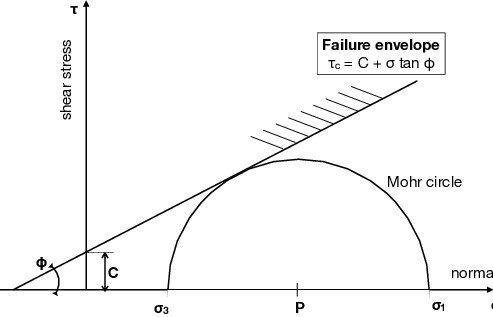
\includegraphics[width=0.5\linewidth]{./pic/The-Mohr-Coulomb-failure-criteria-and-Mohrs-circle.png}
    		\caption{Mohr-Coulomb circle}
    		\label{fig: Mohr-Coulomb circle}
    	\end{figure}
    	\vspace{-5mm}
    	Acorrding to the Mohr-Coulomb circle, we have:
    	
    	\vspace{-2mm}
    	\begin{equation}
    		\frac{\sigma_1}{\sigma_3} = \frac{1+\sin \phi}{1-\sin \phi}
    	\label{eq: mohr circle}
    \end{equation}

	\vspace{-2mm}
    	In the model of MCC, the critical stress ratio $M = \frac{q}{p}$ can be represented as:
    	
    	\vspace{-2mm}
    	\begin{equation}
    		\left \{ \begin{aligned}
    			&M_{compression}= \frac{\sigma_1 - \sigma_3}{(\sigma_1+2\sigma_3)/3} = \frac{6\sin \phi}{3-\sin \phi}\\
    			&M_{extension}= \frac{\sigma_1 - \sigma_3}{(2\sigma_1+\sigma_3)/3} = \frac{6\sin \phi}{3+\sin \phi}
    		\end{aligned} 
    		\right.
    		\label{eq: M calculation}
    	\end{equation}
    \end{minipage}
\end{frame}

\begin{frame}
	\fontsize{8}{8}\selectfont
	\begin{minipage}{0.5\linewidth}
	SMP failure criterion:
	\begin{equation}
		\left \{ \begin{aligned}
			\frac{I_1I_2}{I_3} &\leq \mathrm{const.}  \\
			\mathrm{const.} &= \frac{\left(\sigma_{1}+2 \sigma_{3}\right)\left(2 \sigma_{1} \sigma_{3}+\sigma_{3}^{2}\right)}{\sigma_{1} \sigma_{3}^{2}} \\ 
			&= \frac{9-\sin^2 \phi}{1-\sin^2 \phi}\\		
			q_{c}&=\frac{2 I_{1}}{3 \sqrt{\left(I_{1} I_{2}-I_{3}\right) /\left(I_{1} I_{2}-9 I_{3}\right)}-1}
		\end{aligned}
		\right.
		\label{eq: smp criterion}
	\end{equation} 
	Modified Lade failure criterion:
	\begin{equation}
		\left \{ \begin{aligned}
			& \frac{I_1^3}{I_3} - 27+\eta \leq 0\\
			& \eta = \frac{4\tan^2 \phi (9-7\sin \phi)}{1-\sin \phi}
		\end{aligned}
		\right.
	\end{equation} 
\end{minipage}
\vspace{3mm}
\begin{minipage}{0.47\linewidth}
	\begin{figure}
		\centering
		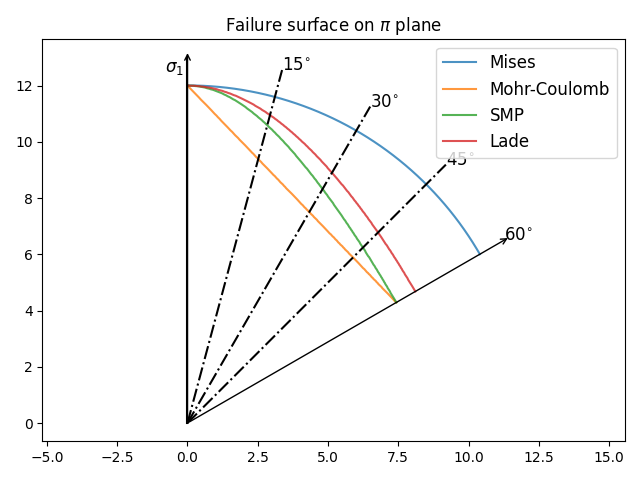
\includegraphics[width=\linewidth]{./pic/yield surface under different criterion.png}
		\caption{Yield surfaces under different criterion on the $\pi$ plane}
		\label{fig: yield surfaces}
	\end{figure}
\end{minipage}

The Mises can be transformed to SMP through the paper\footnote{Matsuoka H, Yao YP, Sun D (1999) The Cam-clay models revised by the SMP criterion.}.
\end{frame}

\begin{frame}{Yield surfaces in 3D space}
\begin{figure}
	
	\centering
	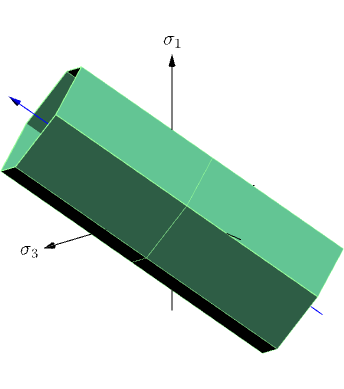
\includegraphics[width=0.15\linewidth]{./pic/tresca 3d.png}
	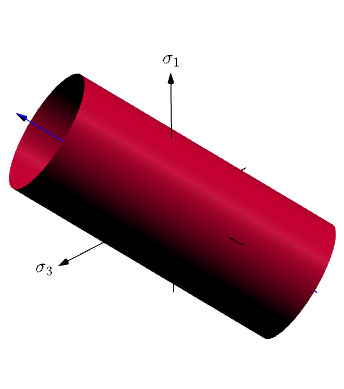
\includegraphics[width=0.15\linewidth]{./pic/von-mises 3d.png}
	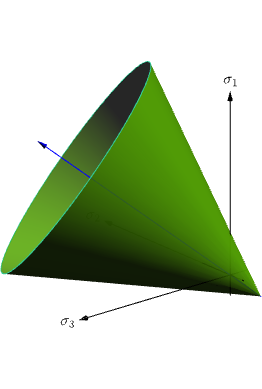
\includegraphics[width=0.1125\linewidth]{./pic/drucker-prager 3d.png}
	\caption{(a)Tresca surface; (b)Von-mises surface; (c)Drucker-Prager surface}
	\label{fig: (a)Tresca surface; (b)Von-mises surface; (c)Drucker-Prager surface}
\end{figure}

\vspace{-5mm}
\begin{figure}
	\centering
	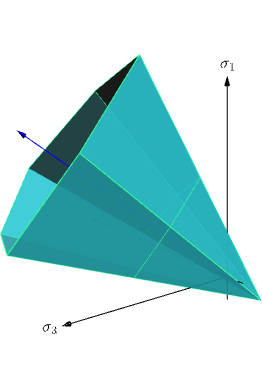
\includegraphics[width=0.15\linewidth]{./pic/mohr-coulomb 3d.png}
	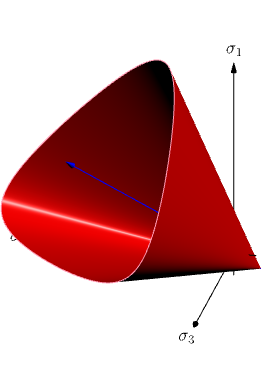
\includegraphics[width=0.15\linewidth]{./pic/smp 3d.png}
	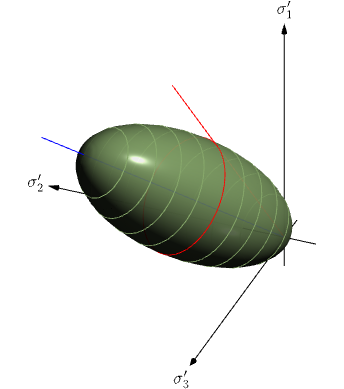
\includegraphics[width=0.2\linewidth]{./pic/mcc yield surface.png}
	\caption{(a)Mohr-Coulomb surface; (b)SMP surface; (c)MCC surface}
	\label{fig: mohr smp mcc}
\end{figure}

\end{frame}

\subsection{Hardening model}

\begin{frame}{Hardening model}
    There are many hardening models, as the plastic strain or the plastic energy used as the internel variables.
    \begin{itemize}
        \item Exponential hardening model (generally used for metals)
        \begin{equation}
            H=A+B(\epsilon_0+\epsilon_{s}^{p})^n
            \label{eq: exponential hardening model}
        \end{equation}
        
        \item Maximum of the mean pressure (MCC and OCC) models, and a series extended model based on the MCC model
        \begin{equation}
            \left\{\begin{matrix}
                H = \frac{\epsilon_v^p}{c_p}\\
                c_p = \frac{\lambda-\kappa}{1+e_0}
            \end{matrix}\right.
            \label{eq: maximum mean pressure}
        \end{equation}
        
    \end{itemize}
\end{frame}

\subsection{Flow rules (Plastic energy function)}
\begin{frame}{Flow rules}
    The fLow rules decide the direction of the plastic strain in the plastic return mapping calculation, which is used to make sure the stress still on the yield function once loading into plastic stage.
    
    \vspace{0.2cm}
    The flow rules can be generally summarised as:
    \begin{itemize}
        \item associated 
        \item non-associated
    \end{itemize}
    
    \vspace{0.2cm}
    Actually, in the most widely used elastoplastic models, the associated flow rule is employed.
    
    \vspace{0.2cm}
    The yield function $f(\sigma_{ij}, H)$ decides the stress stress while the plastic energy function $g(\sigma_{ij})$ governs the direction of plastic deformation through:
    \begin{equation}
    \mathrm{d}\epsilon_{ij}^{p}=\mathrm{d}\lambda \frac{\partial g}{\partial \sigma_{ij}}
    \label{eq: plastic flow}
    \end{equation}
\end{frame}

\section{MCC model}
\begin{frame}{MCC model}
    In the MCC model, at first, we need to use the consolidation line to describe the link between void ratio and the consolidation pressure (mean stress $p\ (\mathrm{kPa})$).
    \vspace{0.2cm}
    
    \begin{minipage}[c]{0.58\linewidth}
        The consolidation line: 
        \vspace{-2mm}
        \begin{equation}
            v = v_{\lambda}-\lambda\ln{\frac{p}{p_1}}
            \label{eq: consolidation line}
        \end{equation}
        \vspace{-1mm}
        And the swelling line:
        \vspace{-2mm}
        \begin{equation}
            v = v_{\kappa}-\kappa\ln{\frac{p}{p_1}}
            \label{eq: swelling line}
        \end{equation}
        \vspace{-1mm}
        According to this line we can calculate the elastic bulk modulus:
        \vspace{-2mm}
        \begin{equation}
            K = \frac{\mathrm{d}p}{\mathrm{d}\epsilon_v}=\frac{p(1+e)}{\kappa}
            \label{eq: elatic modulus calculation in }
        \end{equation}
    \end{minipage}
    \hspace{3mm}
    \begin{minipage}[c]{0.38\linewidth}
        \centering
        \begin{figure}
            \centering
            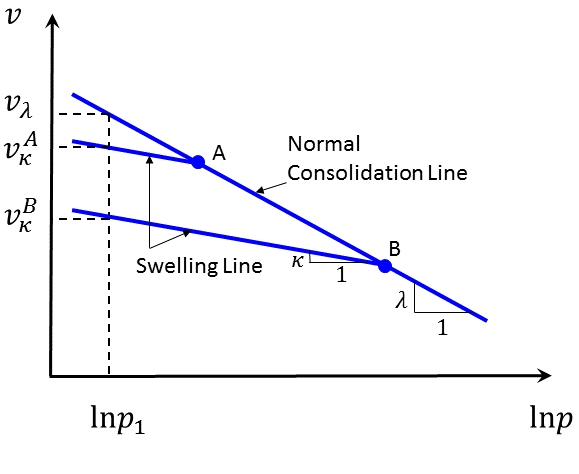
\includegraphics[width=5cm]{./pic/normal consolidation.png}
            \caption{Normal consolidation line}
            \label{fig: normal consolidation}
        \end{figure}
    \end{minipage}
\end{frame}


\begin{frame}{MCC model}
    \begin{minipage}[c]{0.55\linewidth}
        The yield function of MCC; because of the associated flow rule, the plastic energy function equals to yield function:
        \begin{equation}
            f(q, p, p_c)=g(q, p) = q^2+M^2 p(p-p_c)
            \label{eq: mcc yield function}
        \end{equation}
        Then we get the direction of the plastic deformation once the material is loaded into plastic stage:
        \begin{equation}
            \mathrm{d} \epsilon_{ij}^p=\mathrm{d}\lambda\frac{\partial g}{\partial \sigma_{ij}}
            \label{eq: plastic deformation calculation in mcc}
        \end{equation}
    \end{minipage}
    \hspace{3mm}
    \begin{minipage}[c]{0.4\linewidth}
        \centering
        \begin{figure}
            \centering
            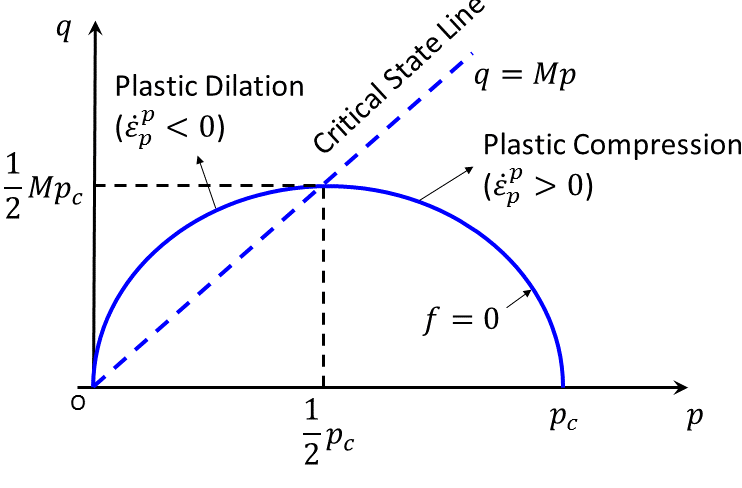
\includegraphics[width=5cm]{./pic/yield function in p-q space.png}
            \caption{Yield function of the MCC model}
            \label{fig: yield function of the mcc model}
        \end{figure}
    \end{minipage}
\end{frame}

\begin{frame}{MCC model: plastic return mapping}
    Then comes to the return mapping caculation. 
    \vspace{2mm}
    According to the consistent condition:
    \begin{equation}
        \mathrm{d}f = \frac{\partial f}{\partial \sigma_{ij}}\mathrm{d}\sigma_{ij}+\frac{\partial f}{\partial H}\frac{\partial H}{\partial \epsilon_{ij}^{p}}\mathrm{d}\epsilon_{ij}^{p}=0
        \label{eq: consistent condition}
    \end{equation}
    Substituting Eq. (\ref{eq: plastic deformation calculation in mcc}) into Eq. (\ref{eq: consistent condition}):
    \begin{equation}
        \frac{\partial f}{\partial \sigma_{ij}}D^{e}_{ijkl}(\mathrm{d}\epsilon_{ij}-\mathrm{d}\lambda\frac{\partial g}{\partial \sigma_{ij}})+\frac{\partial f}{\partial H}\frac{\partial H}{\partial \epsilon_{ij}^{p}} \mathrm{d}\lambda\frac{\partial g}{\partial \sigma_{ij}}=0
        \label{eq: consistent condition 2}
    \end{equation}
    Then we can derive the plastic scaler $\mathrm{d} \lambda$ as following:
    \begin{equation}
        \mathrm{d}\lambda = \frac{\frac{\partial f}{\partial \sigma_{ij}} D^{e}_{ijkl} \mathrm{d} \epsilon_{kl} } {\frac{\partial f}{\partial \sigma_{ij}} D^{e}_{ijkl} \frac{\partial g}{\partial \sigma_{kl}} - \frac{\partial f}{\partial H}\frac{\partial H}{\partial \epsilon_{ij}^{p}}\frac{\partial g}{\partial \sigma_{ij}}}
        \label{eq: dlambda calculation}
    \end{equation}
\end{frame}

\begin{frame}{MCC model: plastic return mapping}
    With $\mathrm{d}\lambda$ we can calculate the plastic strain:
    \begin{equation}
        \mathrm{d} \epsilon_{ij}^p = \mathrm{d} \lambda \frac{\partial g}{\partial \sigma_{ij}}
        \label{eq: plastic strain calculation}
    \end{equation}
    And the stress: 
    \begin{equation}
        \mathrm{d} \sigma_{ij} = D^{e}_{ijkl}(\mathrm{d} \epsilon_{kl} - \mathrm{d} \epsilon_{kl}^p)
        \label{eq: stress calculation after plastic deformation calculation}
    \end{equation}
    Substituting Eq. (\ref{eq: dlambda calculation}) and Eq. (\ref{eq: plastic strain calculation}) into Eq. (\ref{eq: stress calculation after plastic deformation calculation}), we get:
    \begin{equation}
        \mathrm{d} \sigma_{ij} = D^{e}_{ijkl}(\mathrm{d} \epsilon_{kl} - \frac{\frac{\partial f}{\partial \sigma_{mn}} D^{e}_{mnst} \mathrm{d} \epsilon_{st} } {\frac{\partial f}{\partial \sigma_{mn}} D^{e}_{mnst} \frac{\partial g}{\partial \sigma_{st}} - \frac{\partial f}{\partial H}\frac{\partial H}{\partial \epsilon_{mn}^{p}}\frac{\partial g}{\partial \sigma_{mn}}} \frac{\partial g}{\partial \sigma_{kl}})
    \end{equation}  
    \label{eq: stress calculation after plastic deformation calculation 2}
\end{frame}

\begin{frame}{MCC model: plastic return mapping}
    In Eq. (\ref{eq: stress calculation after plastic deformation calculation 2}) after assuming the subscripts in tensor $\mathrm{d} \epsilon_{st} \rightarrow \mathrm{d} \epsilon_{kl}$ and $\frac{\partial g}{\partial \sigma_{kl}} \rightarrow \frac{\partial g}{\partial \sigma_{st}}$, the elastoplastic matrix can be presented as:
    \begin{equation}
        \left\{\begin{array}{l}
            D^{ep}_{ijkl} = D^{e}_{ijkl} \left(1- \frac{\frac{\partial f}{\partial \sigma_{mn}} D^{e}_{mnst} \frac{\partial g}{\partial \sigma_{st}} } {\frac{\partial f}{\partial \sigma_{mn}} D^{e}_{mnst} \frac{\partial g}{\partial \sigma_{st}} - \frac{\partial f}{\partial H}\frac{\partial H}{\partial \epsilon_{mn}^{p}}\frac{\partial g}{\partial \sigma_{mn}}}\right) \\
            \mathrm{d} \sigma_{ij} = D^{ep}_{ijkl}\mathrm{d} \epsilon_{kl}
        \end{array}\right.
        \label{eq: elastoplastic material matrix}
    \end{equation}
    \textbf{Note:} because of the assumptions, $D^{ep}_{ijkl}\mathrm{d}\epsilon_{kl} \neq D^{e}_{ijkl}\left(\mathrm{d}\epsilon_{kl} - \mathrm{d}\epsilon_{kl}^p \right)$. \textbf{According to my experience, the stress increment calculated as Eq. (\ref{eq: stress calculation after plastic deformation calculation}) will benefit the nonlinear iteration in the FEM calculation because of it is the accurate value without assumptions.}
\end{frame}

\begin{frame}{MCC model: plastic return mapping}
    \begin{minipage}{0.55\linewidth}
        Followed by the plastic return mapping calculation, the internal variable ($p_c$) in the MCC model should be renewed:
        \begin{equation}
            \mathrm{d}p_c = \exp{ \left (\frac{(1+e)\mathrm{d}\epsilon_{ii}^{p}}{\lambda-\kappa}\right)}p_c-p_c
            \label{eq: pc renewation in MCC model}
        \end{equation}
        \textbf{That's how to calculate the stress while yielding and update the yield surface.}
    \end{minipage}
    \hspace{2mm}
    \begin{minipage}{0.40\linewidth}
        \begin{figure}
            \centering
            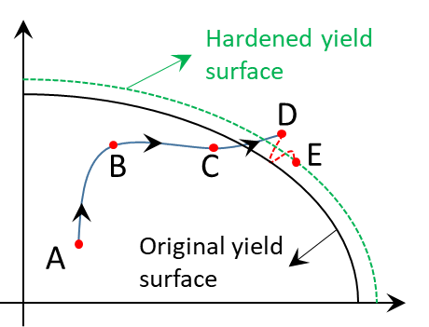
\includegraphics[width=\linewidth]{./pic/plastic return mapping.png}
            \caption{Schematic of the plastic return mapping }
            \label{fig: plastic return mapping}
        \end{figure}
    \end{minipage}
\end{frame}

\section{UH model}
\begin{frame}{UH model}
    \begin{minipage}{0.58\linewidth}
        The MCC model, concentrated on the clay, can not reproduce the dilation of the frictional materials due to the non-negtive dilation angle as is shown in Eq. (\ref{eq: dilation angle of the MCC model}). 
        \begin{equation}
            \frac{\mathrm{d}\epsilon_{ii}^p}{\mathrm{d}\epsilon_{s}^p} = \frac{M^2-\eta^2}{2\eta}
            \label{eq: dilation angle of the MCC model}
        \end{equation}
        \vspace{-1mm}
        Such as the dense sand which will swell under the conventional drained odometer test. As also controlled by the friction, rockfills will dilate if the initial state is dense enough. 
        
        \vspace{2mm}
        So here introduced Yao's work about the Unified Hardening method to construct the unified hardening rule for both clay and sands\cite{Yao2019}.
    \end{minipage}
    \hspace{2mm}
    \begin{minipage}{0.38\linewidth}
        \begin{figure}
            \centering
            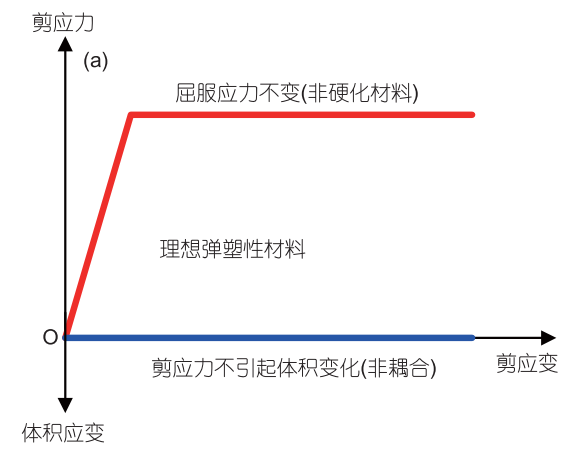
\includegraphics[width=0.48\linewidth]{./pic/ideal elastic-plastic material.jpg}
            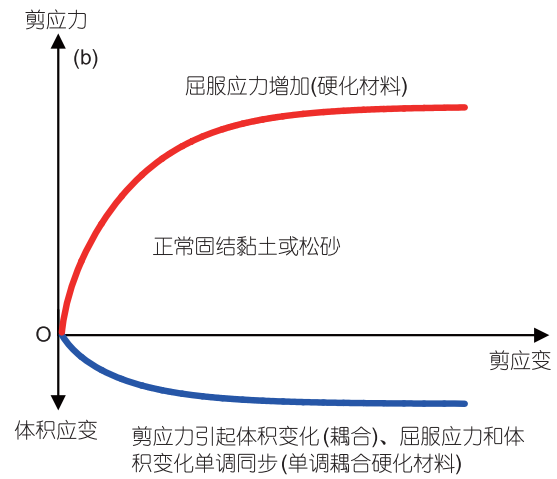
\includegraphics[width=0.48\linewidth]{./pic/dense sand or clay.jpg}
            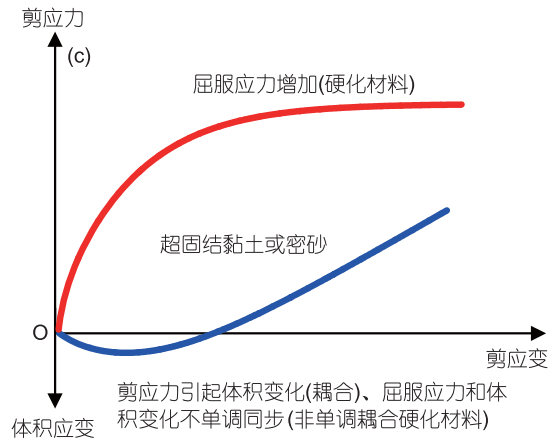
\includegraphics[width=0.55\linewidth]{./pic/dense sand.jpg}
            \caption{Compression comparison between loose and dense sands}
            \label{fig: sand and clay compression}
        \end{figure}
    \end{minipage}
\end{frame}

\begin{frame}{UH model}
    % \fontsize{9}{9}\selectfont
    Compared with the yield function of MCC model Eq. (\ref{eq: mcc yield function}), the key modification is on the hardening variables, as is shown in following equation:
    \begin{equation}
        \left\{\begin{aligned}
            &f=g=\ln \frac{p}{p_{0}}+\ln \left(1+\frac{q^{2}}{M^{2} p^{2}}\right)-\frac{H}{c_{\mathrm{p}}}=0 \\
            &c_p = \frac{1+e}{\lambda - \kappa}\\
            &H_{MCC}=\varepsilon_{\mathrm{v}}^{\mathrm{p}}\\
            &H_{UH} = \int c(p, q) \mathrm{~d} \varepsilon_{\mathrm{v}}^{\mathrm{p}} = \int \frac{M^{4}}{M_{\mathrm{f}}^{4}} \frac{M_{\mathrm{f}}^{4}-\eta^{4}}{M^{4}-\eta^{4}} \mathrm{~d} \varepsilon_{\mathrm{v}}^{\mathrm{p}}
        \end{aligned}\right.
        \label{eq: yield function in UH model}
    \end{equation}
\end{frame}

\begin{frame}{UH model}
    \fontsize{10}{9}\selectfont
    \begin{minipage}[c]{0.48\linewidth}
        In the MCC model we have:
    \begin{equation}
        \left\{
            \begin{aligned}
                    &\frac{\partial g}{\partial p} = \frac{2M^2p}{M^2p^2+q^2}-\frac{1}{p}\\
                    &\frac{\partial g}{\partial q} = \frac{2q}{M^2p^2+q^2}\\
                    &\frac{\mathrm{d}\epsilon_{ii}^p}{\mathrm{d}\epsilon_{s}^p} = \frac{\partial g}{\partial p}/\frac{\partial g}{\partial p} = \frac{M^2-\eta^2}{2\eta}\\
                    &\mathrm{d} \lambda = c_p \left( \mathrm{d} p + \frac{2\eta}{M^2-\eta^2}\mathrm{d}q\right)
            \end{aligned}
        \right.
        \label{eq: plastic direction in the MCC model}
    \end{equation}
    \end{minipage}
    \vspace{2mm}
    \begin{minipage}[c]{0.50\linewidth}
        After introduced the UH hardening:
        \begin{equation}
        \left\{
            \begin{aligned}
                    &\frac{\partial g}{\partial p} = \frac{2M^2p}{M^2p^2+q^2}-\frac{1}{p}\\
                    &\frac{\partial g}{\partial q} = \frac{2q}{M^2p^2+q^2}\\
                    &\mathrm{d} \lambda = \frac{c_p}{c(p, q)}  \left(\mathrm{d}p+\frac{2\eta}{M^2-\eta^2}\mathrm{d}q\right)\\
                    &c\left(p, q\right)=\frac{M^{4}}{M_{\mathrm{f}}^{4}} \frac{M_{\mathrm{f}}^{4}-\eta^{4}}{M^{4}-\eta^{4}}
            \end{aligned}
        \right.
        \label{eq: plastic direction in the UH model}
    \end{equation}
    \end{minipage}
    
    The dilation angle are the same, while the plastic scaler $\mathrm{d} \lambda$ is changed. \textbf{The scaler can be negative once the stress ratio $\eta = \frac{q}{p}$ is larger than the critical stress ratio $M$, which agrees with the phenomenan that the dilation always happen along with the stress peak.}
\end{frame}

\section{CSUH model}

\begin{frame}{CSUH model: highlights}
    Based on the UH model, some further modifications were carried out to implement the CSUH model \cite{UHmodelYao2019b}. There are several main points in the CSUH model, compared with the UH model:
    \begin{itemize}
        \item Non-association flow through a newly-introduced variable $M_c$ to control the dilation;
        \item Internal variable $\xi$ to represent the current stage according to the ACL (Anisotropic compression line);
        \item A curved line representing the $e-\ln{p}$ relationship;
        \item An parameter $\chi$ to involved to describe the distance between NCL and CSL.
        \item Transformed stress space used to consider the medium principal stress coefficient $b = \frac{\sigma_2 - \sigma_3}{\sigma_{1}-sigma_{3}}$
    \end{itemize}
\end{frame}

\begin{frame}{CSUH model: Non-association}
    \fontsize{10}{10}\selectfont
    \begin{minipage}[c]{0.50\linewidth}
        Different from the associated flow rule in the MCC model, a variable $M_c$ is introduced to construct the energy function:
    \begin{equation}
        g = \ln{p} + \ln{\left( 1+ \frac{q^2}{M_c^2 p^2}\right)}
        \label{eq: energy function in the CSUH model}
    \end{equation}
    where, $M_c=M\exp\left({-m\xi}\right)$, $M$ is the critical stress ratio, $\xi$ is the variable representing the material state, and $m$ is the material constant calibrated through \textbf{undrained compression test} regarding:
    \begin{equation}
        m=-\frac{1}{\xi_c}\ln{\frac{M_c^{\xi_c}}{M}}
        \label{eq: material constant m calibration}
    \end{equation}
    \end{minipage}
    \hspace{10mm}
    \begin{minipage}{0.4\linewidth}
        \begin{figure}
            \centering
            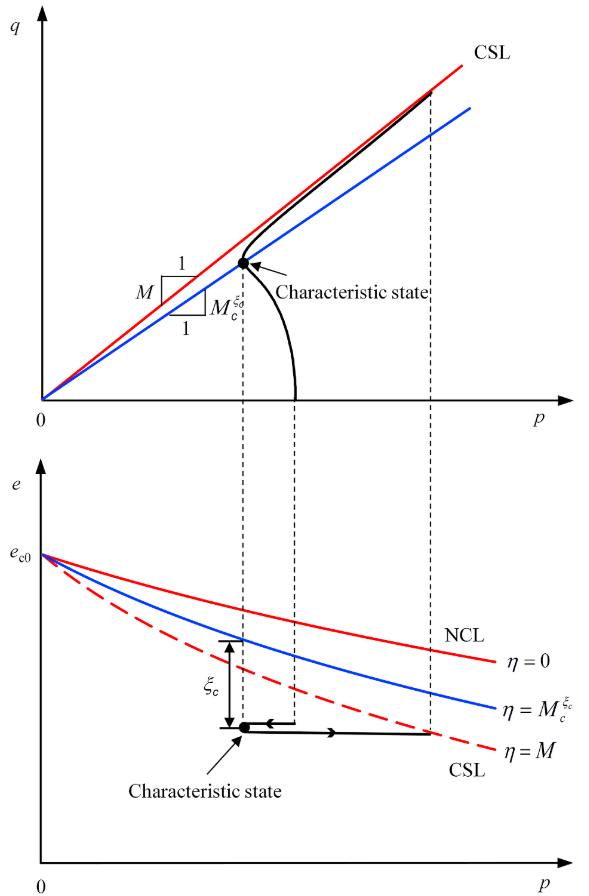
\includegraphics[width=0.7\linewidth]{./pic/m calibration.jpg}
            \caption{Material constant $m$ calibration}
            \label{fig: m calibration}
        \end{figure}
    \end{minipage}
\end{frame}

\begin{frame}{CSUH: internal variable $\xi$}
    \begin{minipage}[c]{0.58\linewidth}
        Variable $\xi$ is used for representing the current stage of the material. According to Fig. (\ref{fig: e_eta calcualtion}), we can calculate the $e_{\eta}$ wrt the current stress ratio $\eta = q/p$ and the functions of the lines:
        \begin{equation}
            \left\{\begin{aligned}
                &e_{\eta}=N-\lambda \ln p-(\lambda-\kappa) \ln \left(1+\frac{\eta^{2}}{M^{2}}\right) \\
                &\xi = e_{\eta}-e
            \end{aligned}\right.
            \label{eq: e_eta calculation}
        \end{equation}
        \textbf{$\xi$ is very important in this model.} There are 2 kinds of conditions of the current stages:
        \begin{itemize}
            \item $\xi > 0$: Current material is \textcolor{red}{denser} than the corresponding CS (Critical state);
            \item $\xi < 0$: Current material is \textcolor{red}{looser}.
        \end{itemize}
    \end{minipage}
    \hspace{2mm}
    \begin{minipage}[c]{0.38\linewidth}
        \begin{figure}
            \centering
            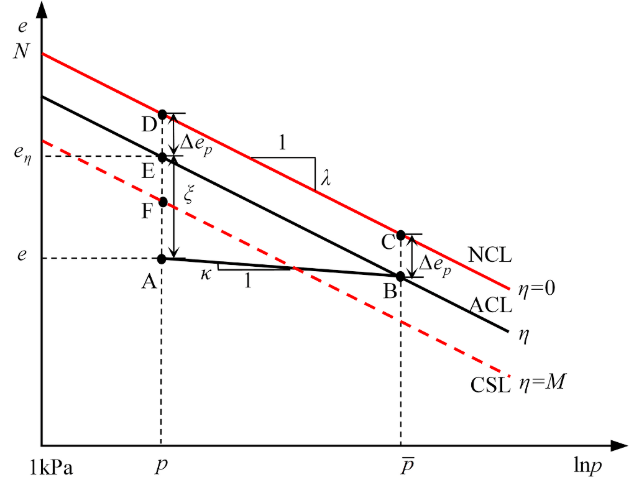
\includegraphics[width=\linewidth]{./pic/e_eta calculation.jpg}
            \caption{$e_{\eta}$ and $\xi$ calculation}
            \label{fig: e_eta calcualtion}
        \end{figure}
    \end{minipage}
\end{frame}

\begin{frame}{CSUH: internal variable $\xi$}
    $\xi$ is the only state variable involved to calculate the failure stress ratio $M_f$ and the feature stress ratio $M_c$. 
    \begin{itemize}
        \item $M_f$ representing the failure stress ratio $q/p$ when will the material fails. \textcolor{red}{That's why a peak of stress will emerge in the $\sigma_s - \epsilon_{axial}$ curve};
        \item $M_c$ mainly influences the direction of the plastic deformation, cuz: $$\mathrm{d} \epsilon_v / \mathrm{d} \epsilon_s = \frac{M_c^2-\eta^2}{2\eta}$$ which means that \textcolor{red}{the smaller $M_c$ is, the material is more tend to dilation}.
    \end{itemize}
    Analogous to the varible $\xi$ in this model,  $\varphi$ is defined in Been and Jefferies model \cite{norsandJefferies1993}\footnote{Been and Jefferies, A state parameter for sands. Geotechnique 1985} to represent the vertical distance between the current state and the CSL.
\end{frame}

\begin{frame}{CSUH: curved line in $e-\ln{p}$ space}
    \fontsize{12}{13}\selectfont
    \begin{minipage}{0.62\linewidth}
        Another thing interesting is that the curve $e-\ln{p}$ is not a straigt line in the semi-$\ln{(p)}$ space, especially at the lower stress level state. Subsequently, there employed an important modification to improve the model:
        \begin{equation}
            \left\{\begin{aligned}
                &\mathrm{MCC\  model:}\  &e& = N-\lambda\ln{p}\\
                &\mathrm{CSUH\  model:}\  &e& = Z-\lambda\ln{\left(\frac{p+p_{si}}{1+p_{si}} \right)}
            \end{aligned}\right.
        \end{equation}
        where, $Z$ is the void ratio as $p=1$\si{kPa}. \textcolor{red}{\textbf{Note: in the this paper, the unit of the $p$ in the $e-\ln{p}$ space is \si{kPa}}}. While $p\rightarrow \infty $, we have $N-\lambda\ln{p}= Z-\lambda\ln{\left(\frac{p+p_{si}}{1+p_{si}} \right)}$. Then $p_{si} = \exp{\left( \frac{N-Z}{\lambda}\right)}-1$.
    \end{minipage}
    \hspace{2mm}
    \begin{minipage}{0.33\linewidth}
        \begin{figure}
            \centering
            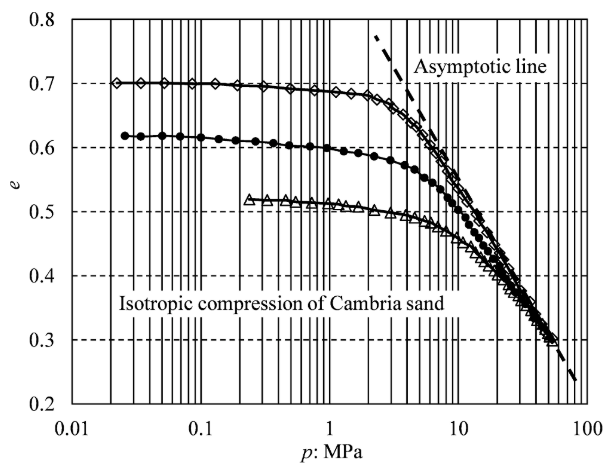
\includegraphics[width=0.85\linewidth]{./pic/Isotropic compression of Cambria sand.jpg}
            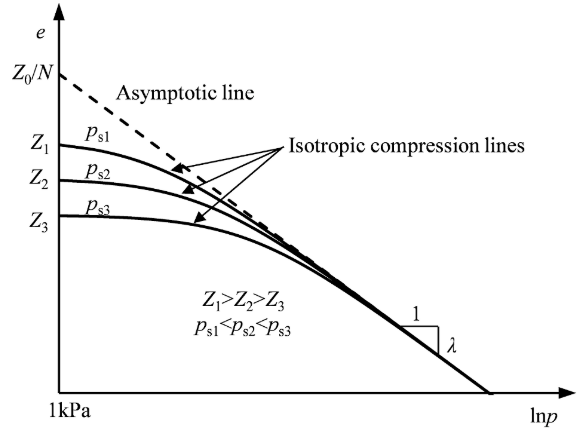
\includegraphics[width=0.85\linewidth]{./pic/different z.jpg}
            \caption{Isotropic compression of Cambria sand}
            \label{fig: Isotropic compression of Cambria sand}
        \end{figure}
    \end{minipage}
\end{frame}

\begin{frame}{CSUH: parameter $\chi$ representing the distance between NCL and CSL}
	\fontsize{9}{9}\selectfont
	\begin{minipage}[c]{0.6\linewidth}
		In the original MCC model, according to the yield function $f=\ln{\frac{p}{p_0}}+\ln{\left(1+\frac{q^2}{M^2p^2}\right)}-\frac{\epsilon_v^p}{c_p}=0$, we can compare \textcolor{red}{the equation in isotropic ($\eta = 0$) and critical state ($\eta=M$)}:
		
		\vspace{-2mm}
		\begin{equation}
			\left\{\begin{aligned}
				&\text{isotropic:} &\ln{\frac{p}{p_0}}&-\frac{\epsilon_{v0}^p}{c_p} = 0\\
				&\text{cirtical state:} &\ln{\frac{p}{p_0}}&+\ln{2} - \frac{\epsilon_{v\eta}^p}{c_p} = 0
			\end{aligned}
			\right.
			\label{eq: distance btween NCL and CSL}
		\end{equation}
	
		\vspace{-2mm}
		As is shown in Fig. (\ref{fig: chi meaning}), the distance grows larger as $\chi$ increase.
		We found the vertical distance between the NCL and the CSL is fixed as $\ln 2$ in the $e-\ln p$ curve. 
		Then a parameter $\chi$ is added to adjust vertical distance between the two lines, and the modified yield function as:
		
		\vspace{-2mm}
		\begin{equation}
			f=\ln \left(\frac{p}{p_0}\right) + \ln\left(\frac{(1+\chi) q^{2}}{M^{2} p^{2}-\chi q^{2}}+1\right)-\frac{\epsilon_v^p}{c_p}=0
			\label{eq: yield function after chi added}
		\end{equation}
	
		\vspace{-2mm}
		\textbf{Then the distance is changed to $\ln \left(2+\chi\right)$.}
	\end{minipage}
	\vspace{2mm}
	\begin{minipage}[c]{0.36\linewidth}
		\begin{figure}
			\centering
			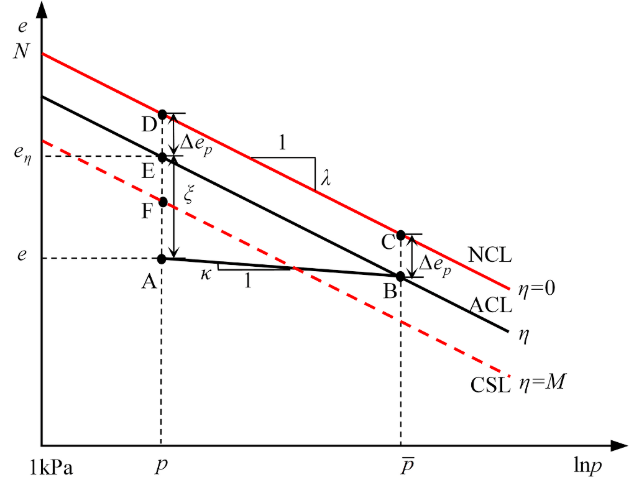
\includegraphics[width=0.7\linewidth]{./pic/e_eta calculation.jpg}
			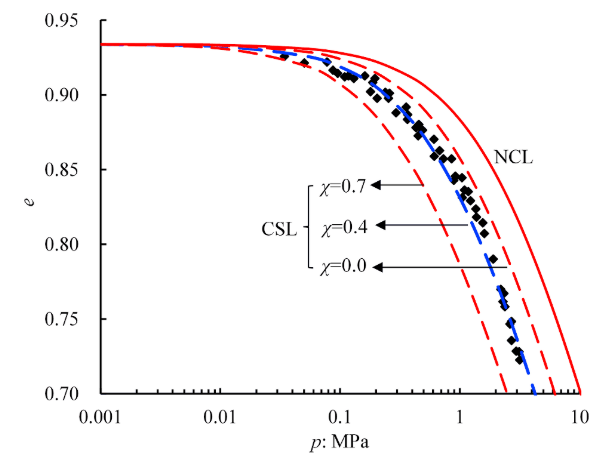
\includegraphics[width=0.75\linewidth]{./pic/csl parameter chi.jpg}
			\caption{CSL parameter $\chi$}
			\label{fig: chi meaning}
		\end{figure}
	\end{minipage}
\end{frame}

\begin{frame}{CSUH model: Transformed stress space based on the SMP criterion}
	\fontsize{9}{9}\selectfont
	To consider the medium stress ratio $b = (\sigma_2-\sigma_3)/(\sigma_1-\sigma_3)$, as is shown in Fig. (\ref{fig: yield surfaces}).
	
	\vspace{2mm}
	\textcolor{red}{\textbf{Without this consideration, the model can not distinguish the compression from the extension}}

\begin{minipage}[c]{0.3\linewidth}
	In the yield function Eq. (\ref{eq: yield function after chi added}), if we calculate $q$ through the Mises stress equation as $q = \sqrt{3J_2}$, the yield surface will be a \textcolor{red}{circle} in the $\pi$ plane. 
	
	\vspace{2mm}
	Then we calculated the $q$ as $q_c$ Eq. (\ref{eq: smp criterion}):
	\begin{equation}
		q_{c}=\frac{2 I_{1}}{3 \sqrt{\left(I_{1} I_{2}-I_{3}\right) /\left(I_{1} I_{2}-9 I_{3}\right)}-1}
	\end{equation} 
\end{minipage}
\hspace{2mm}
\begin{minipage}[c]{0.67\linewidth}
\begin{figure}
	\centering
	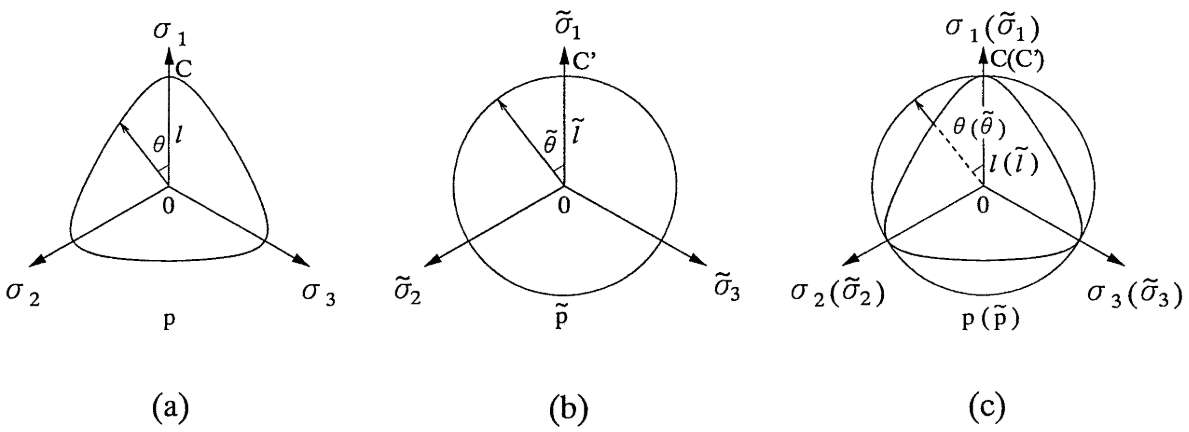
\includegraphics[width=\linewidth]{./pic/transformed space}
	\caption{Transformed stress space}
	\label{fig: transformed-space}
\end{figure}
\end{minipage}
\end{frame}

\section{Tips in FEM subroutine implementation}

\begin{frame}[fragile]{Tips in FEM subroutine implementation}
    \begin{enumerate}
    	\item elasticy and plasticity transformation split
        \item Yield value of the last step added to the $\mathrm{d} \lambda$ calculation
        \item split the loading step as \textit{Abaqus}
        \item \textbf{einsum} method in numpy library 
        \begin{lstlisting}[language=Python]
dsig = np.einsum('ijkl,kl->ij', self.D, deps)
        \end{lstlisting}
    	\item tolerance of the yield value
    \end{enumerate}
\end{frame}

\begin{frame}[fragile]{Tip 1: elastoplastic transformation split}
	Bi-section used in the transformation split:
	\begin{lstlisting}[language=Python,basicstyle=\tiny]
def transformSplit(self, deps):
	rmin, rmax, rmid = 0., 1., 0.5
	sig = self.sigma + np.einsum('ijkl, kl->ij', self.D, deps * rmid)
	p = getP(sigma=sig)
	q = getQ(sigma=sig)
	yieldValue = self.yieldFunction(q=q, p=p, H=self.H, px0=self.px0)
	while True:
		if yieldValue > 0.:
			rmax = rmid
		elif yieldValue < -self.yieldTolerance:
			rmin = rmid
		else:
			break
		rmid = .5 * (rmax + rmin)
		sig = self.sigma + np.einsum('ijkl, kl->ij', self.D, deps * rmid)
		p = getP(sigma=sig)
		q = getQ(sigma=sig)
		yieldValue = self.yieldFunction(q=q, p=p, H=self.H, px0=self.px0)
	return rmid, sig, yieldValue
	\end{lstlisting}
\end{frame}

\begin{frame}[fragile]{Tip 2: yield value in the last return mapping calculation added to current $\mathrm{d} \lambda$}
	Return mapping code based on the CSUH model:
	\begin{lstlisting}[language=Python,basicstyle=\tiny]
def returnMapping(self,):
	e = elast - (1. + elast) * getVolStrain(deps)
	eta_last = q_last / p_last
	# return mapping
	returnMapping_iter = 0
	while True:
		dg_dsigma = self.get_dg_dsigma(Mc=Mc_last, eta=eta_last, 
		                               p=p_last, sigma=sigLast)
		df_dsigma, df_depsvp = self.get_df_dsigma_df_depsp(
		Mf=Mf_last, Mc=Mc_last, sigma=sigLast, p=p_last, q=q_last)
		temp = np.einsum('ij, ijkl, kl->', df_dsigma, Dlast, dg_dsigma) - \
			   df_depsvp * np.trace(dg_dsigma)
		A = (np.einsum('ij, ijkl, kl->', df_dsigma, Dlast, deps) +
		yieldValue_last if yieldValue_last < 1e5 else 0.) / temp
		# A = np.einsum('ij, ijkl, kl->', df_dsigma, Dlast, deps) / temp
		deps_p = A * dg_dsigma
		depsvp = np.trace(deps_p)
		D_ep = Dlast - np.einsum('ijmn, mn, st, stkl->ijkl', Dlast, 
		                         dg_dsigma, df_dsigma, Dlast) / temp
		# sig = sigLast+np.einsum('ijkl, kl->ij', D_ep, deps)
		sig = sigLast + np.einsum('ijkl, kl->ij', Dlast, deps - deps_p)
	\end{lstlisting}
\end{frame}


\begin{frame}[fragile]{Tip 2: yield value in the last return mapping calculation added to current $\mathrm{d} \lambda$}
	\begin{lstlisting}[language=Python,basicstyle=\tiny]
		p = getP(sigma=sig)
		q = getQ(sigma=sig)
		if p < 0.:
			sig = sigLast
			q = q_last
			p = p_last
			deps_p = deps
			depsvp = np.trace(deps_p)
			D_ep = np.zeros_like(self.D)
			xi = xi_last
			H = self.H
			yieldValue = self.yieldFunction(q, p, H, self.px0)
			epsvp = self.epsvp+depsvp
			if self.verboseFlag:
				print('Failed element in the plastic return mapping stage!')
			return sig, q, p, deps_p, D_ep, xi, H, yieldValue, epsvp
		# calculate the updated state variables
		eta= q / p
		xi = self.get_e_eta(eta=eta, p=p) - e
		epsvp = self.epsvp + depsvp
		Mf_last = 0.5 * (Mf_last + self.getM_f(xi))
	\end{lstlisting}
\end{frame}

\begin{frame}[fragile]{Tip 2: yield value in the last return mapping calculation added to current $\mathrm{d} \lambda$}
	\begin{lstlisting}[language=Python,basicstyle=\tiny]
		Mc_last = 0.5 * (Mc_last + self.getM_c(xi))
		eta_last = .5 * (eta_last + eta)
		# K, G, lam = self.getElasticModulus(p=p_last, e=e)
		# Dlast = self.getMaterialMatrix(lam=lam, G=G)
		H = self.H + self.get_dH(
		Mf=Mf_last,
		Mc=Mc_last,
		eta=eta_last, depsvp=depsvp)
		yieldValue = self.yieldFunction(q=q, p=p, H=H, px0=self.px0)
		if np.abs(yieldValue) < self.yieldTolerance:
			if self.verboseFlag:
				print('converged!')
			break
		else:
			if self.verboseFlag:
				print('\t\t\t Yield value: %.3e' % yieldValue)
		returnMapping_iter += 1
		break
	\end{lstlisting}
\end{frame}

\begin{frame}[fragile]{Tip 3: split the loading step as \textit{Abaqus}}
	\begin{lstlisting}[language=Python,basicstyle=\tiny]
while t < loadingStep:
	vel = vel_list[t]
	vel_remain, scaler, remain_du = copy.deepcopy(vel), 1.0, 1.0
	du = Vector(0., Solution(mydomain))
	while True:
		Dbc, Vbc, Nbc = boudaryCondition(loadingPath=loadingPath, nb=nb, fb=fb, vel=vel)
		prob.initialize(f=Nbc, specified_u_mask=Dbc, specified_u_val=Vbc)
		ddu, converge = prob.solve(iter_max=10)
		if converge == False:
			scaler = 0.5 * scaler
		if scaler < 1. / 2 ** 10:
			raise ValueError('=' * 80 + '\n \t Can not converge after 4 times split.' +
			'\n \t please decrease the loading step and retry.')
		vel = 0.5 * vel
		print('\n\t\t Can not converge, original vel_0: %.3e vel_1: %.3e' % (2. * vel, vel))
		else:
			remain_du = remain_du - scaler
			du += ddu
		if remain_du <= 0.:
			break
		t += 1
	disp += du
	\end{lstlisting}
\end{frame}

\begin{frame}{Tip 5: tolerance of the yield value}
	In the mathematical function, we can easily use 0 to split the elasticity and plasticity.
	
	\vspace{2mm} 
	While, in numerical calculation, such as the renewed yieldValue $f$ after the return mapping process can not be exactly zero due to the non-linearity \textcolor{red}{since the derivations ($\frac{\partial f}{\partial \sigma_{ij}}$, $\frac{\partial f}{\partial \epsilon^p_{ij}}$ and $\frac{\partial g}{\partial \sigma_{ij}}$) used is based on last stage}.
	
	\vspace{2mm} 
	So we have to introduce a parameter in the code as the tolerance of the yield value. If the yield value is lower than parameter, the return mapping processure is satisfied. 
\end{frame}

\section{FEM calculation examples}

\begin{frame}{Von-mises model and co-operation with the $\mathcal{NN}$ model}
	\fontsize{9}{9}\selectfont
	Here are the simulating results based on the Von-Mises model Eq. (\ref{eq: vonmises stress}) and exponential hardening Eq. (\ref{eq: exponential hardening model}).
	
	\vspace{5mm}
	\textbf{(a) Mathematical equations; (b) $\mathcal{NN}$ hardening model involed; (c) both hardening model and the Mises stress calculation are substituted by $\mathcal{NN}$.}
	\begin{figure}
		\centering
		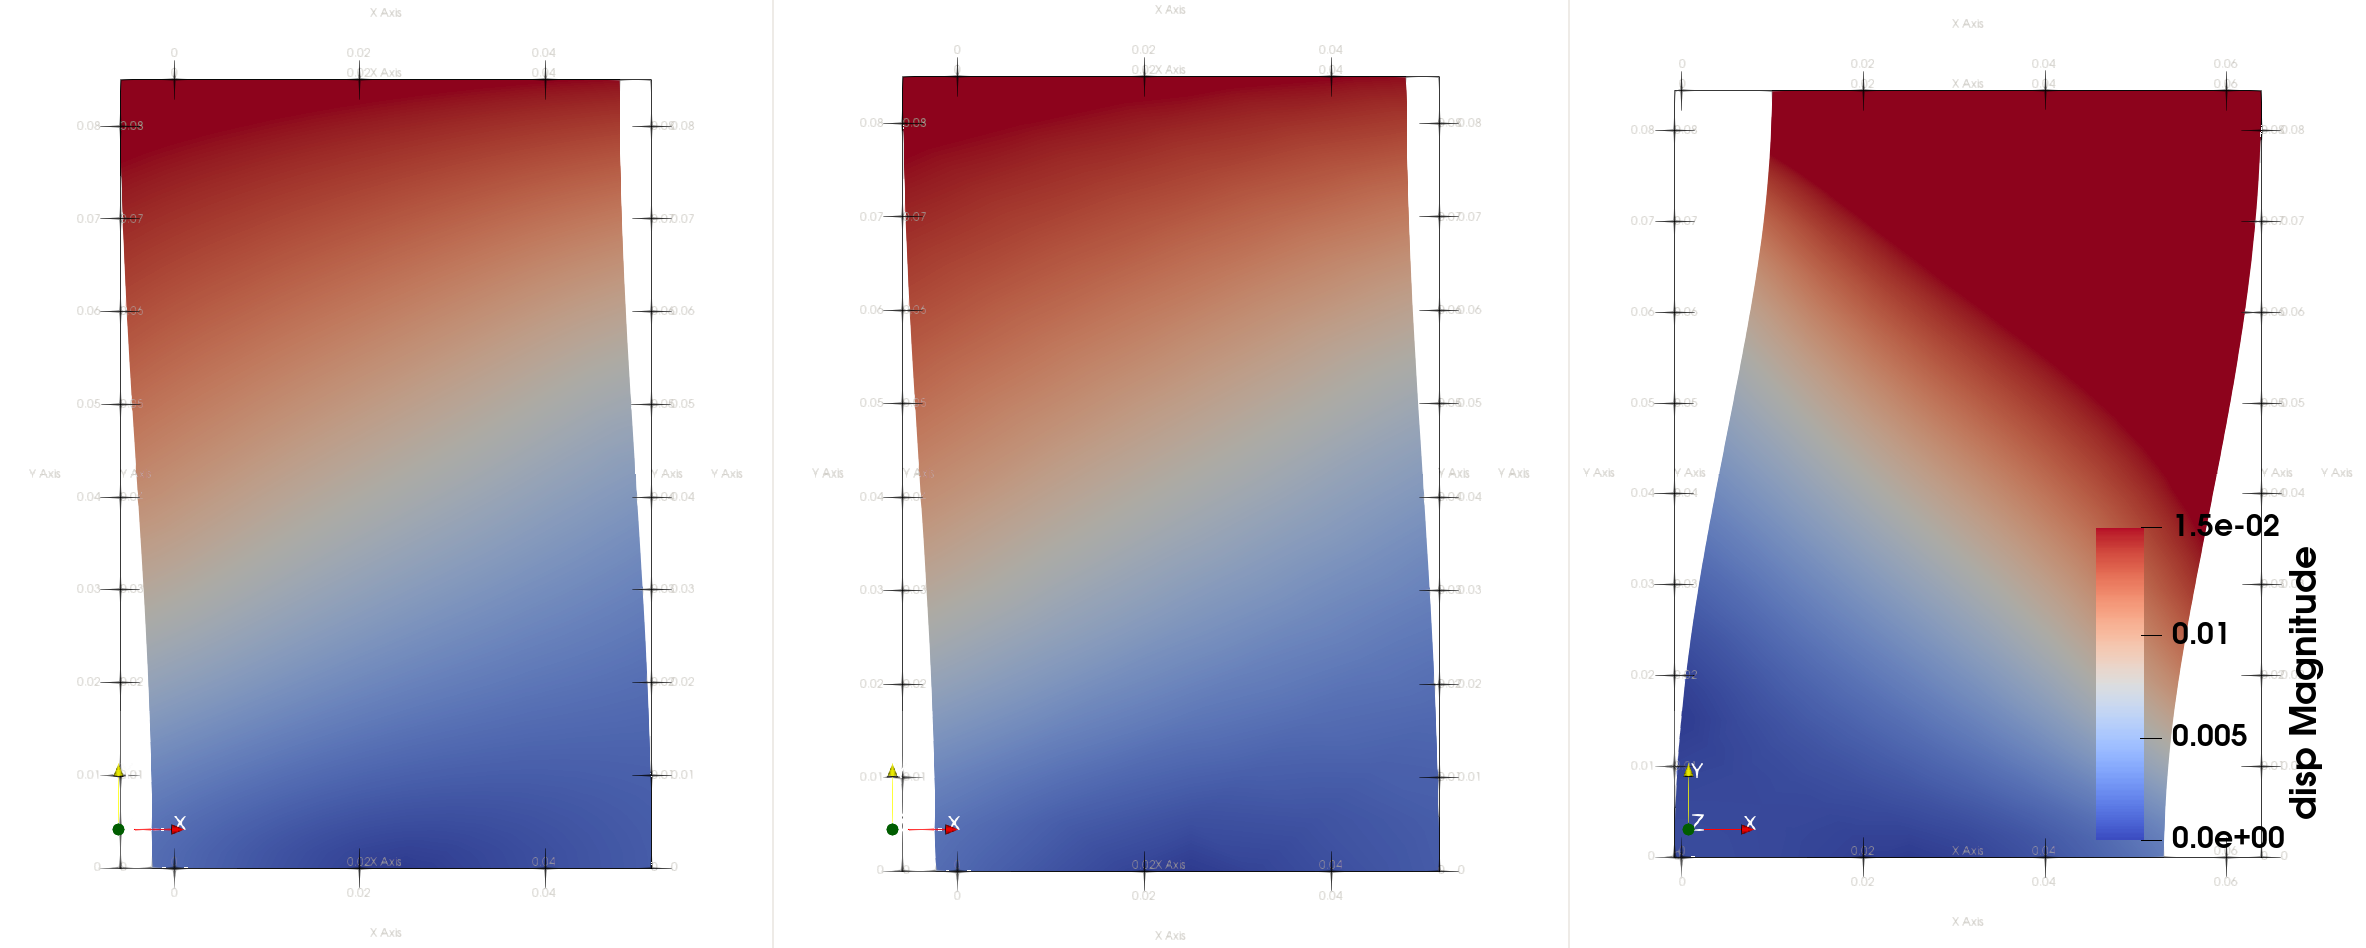
\includegraphics[width=0.6\linewidth]{./pic/mises/displacement.png}
		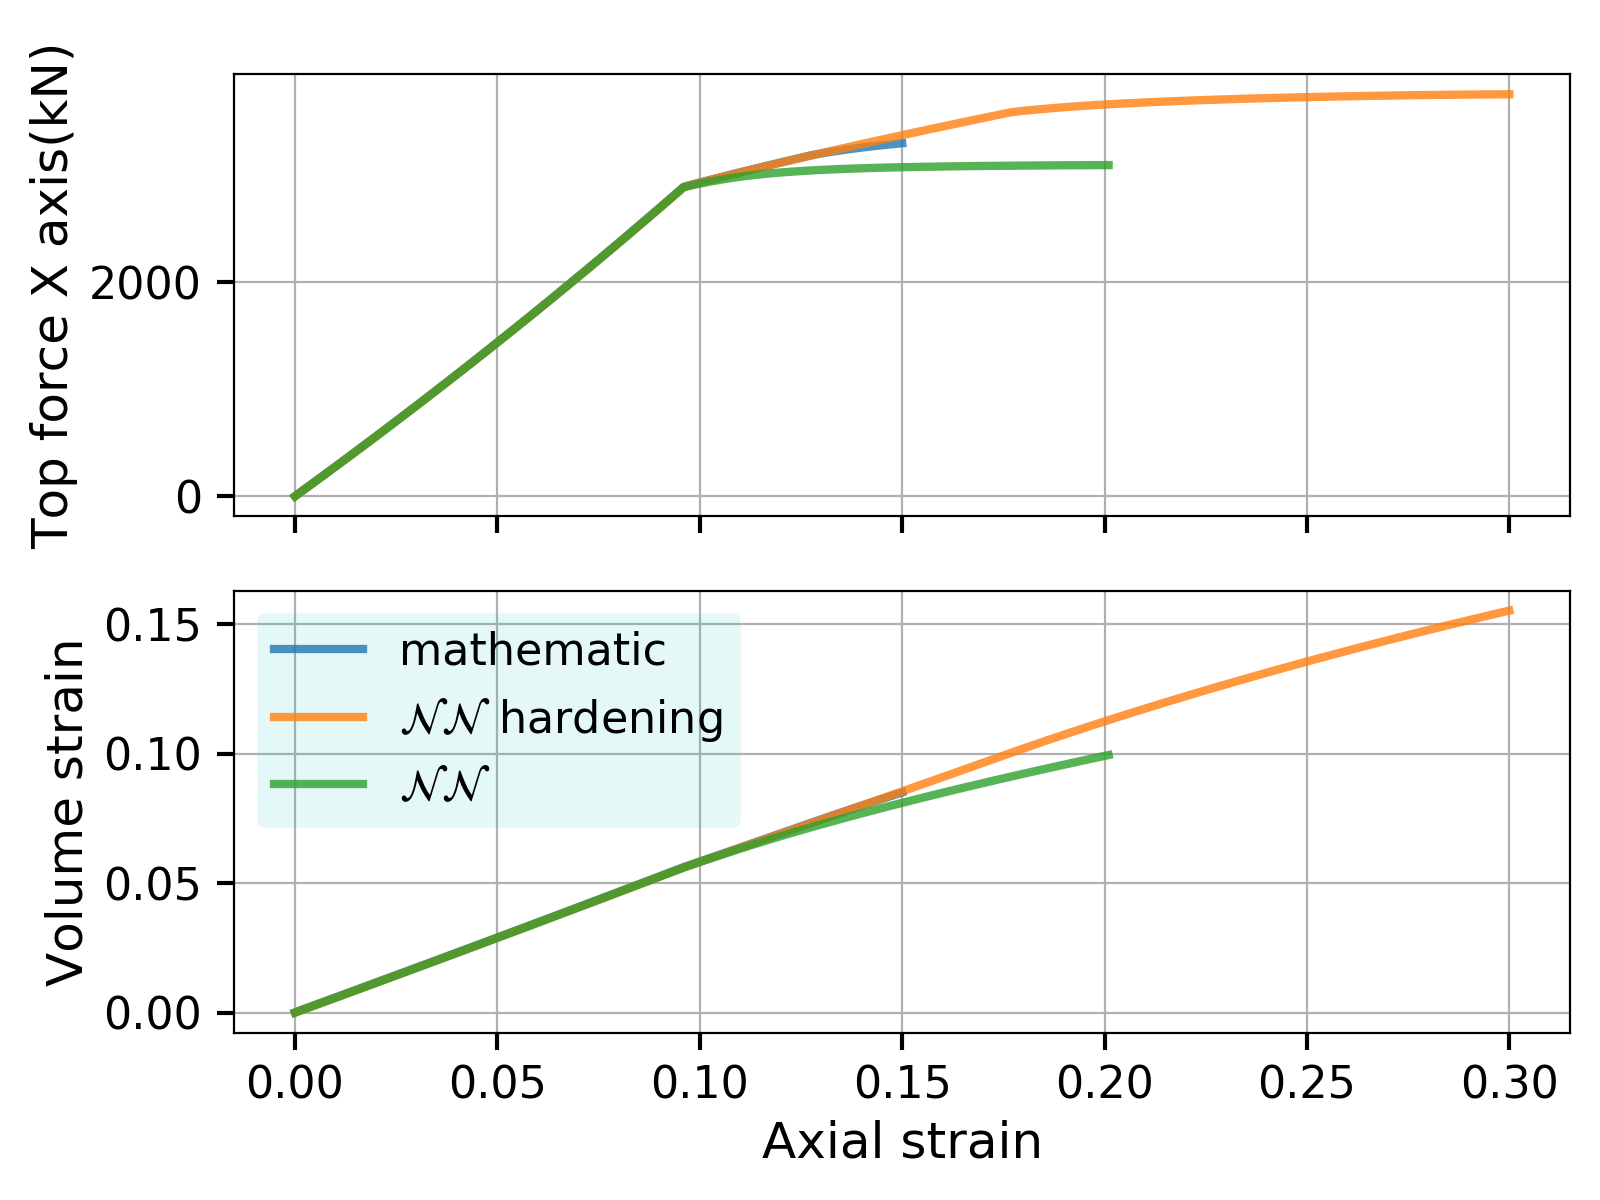
\includegraphics[width=0.35\linewidth]{./pic/mises/footing_Top_force.png}
		\caption{2D calculation based on the Von-Mises model and exponential hardening rule; Top force and volume strain comparison}
		\label{fig: vonmises 2d u}
	\end{figure}
%
%	\begin{figure}
%		\centering
%		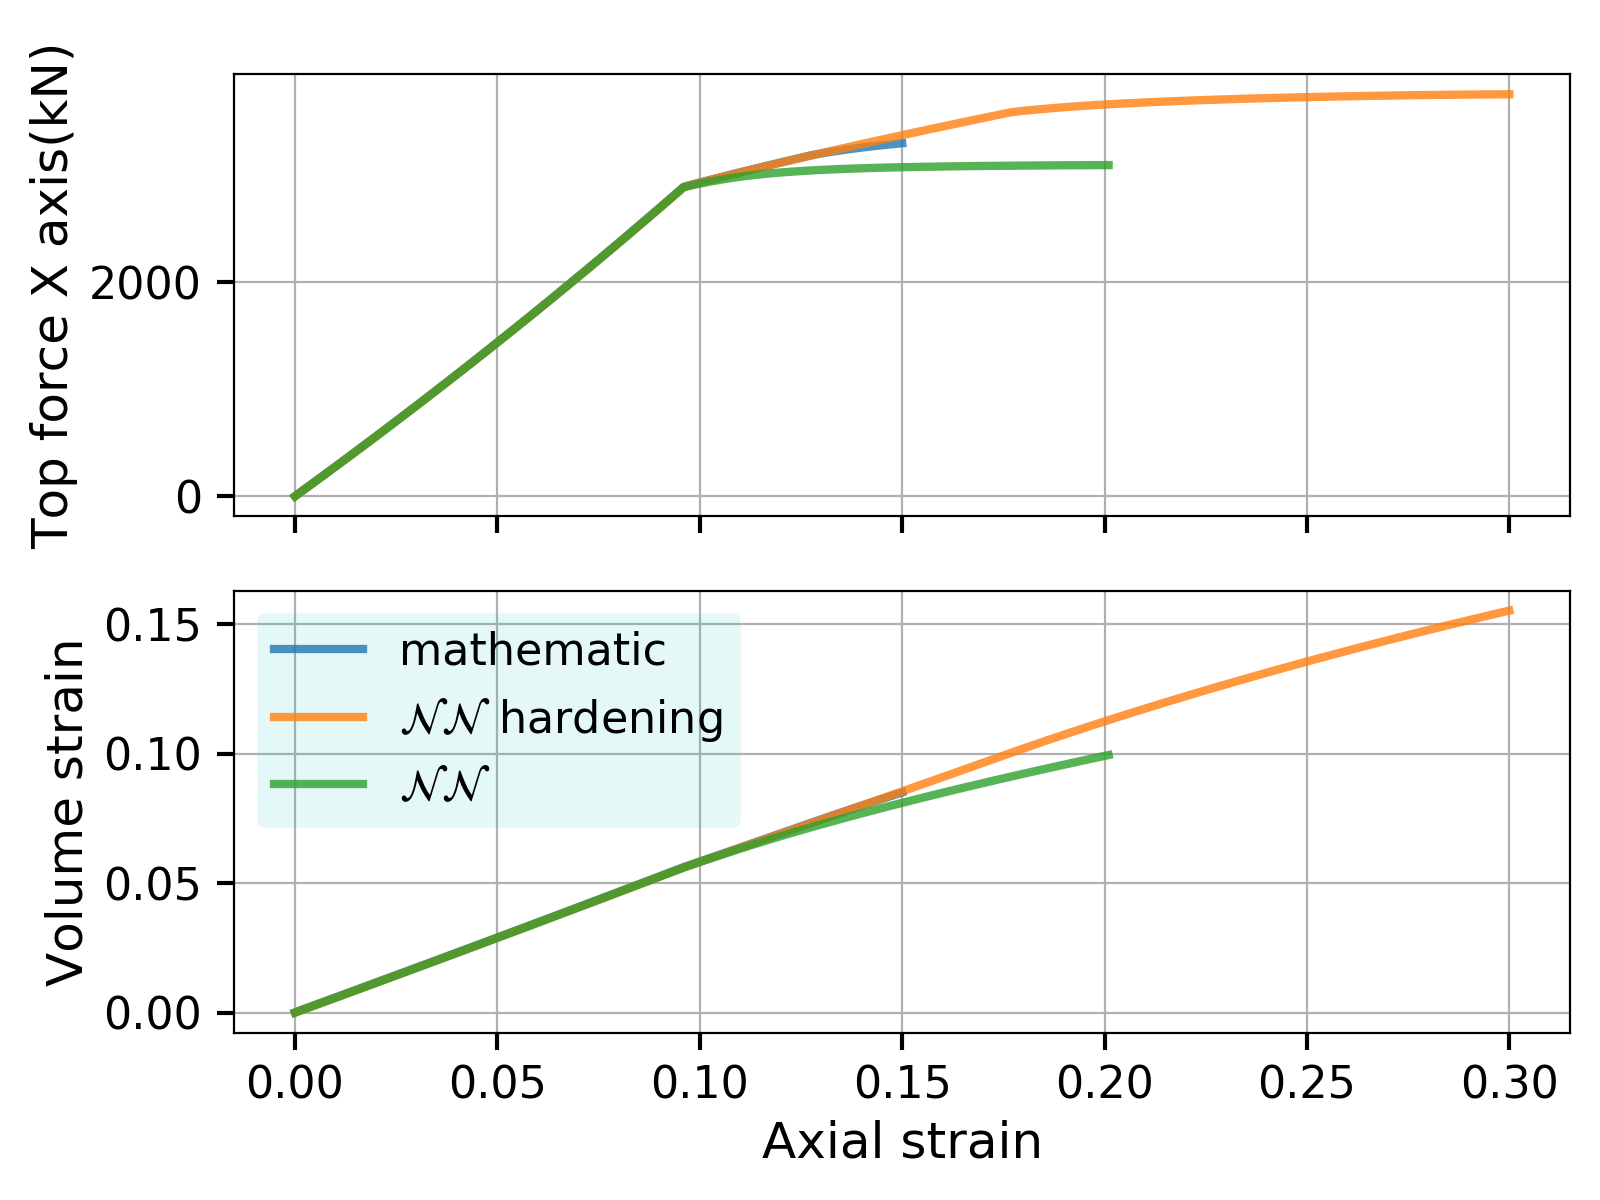
\includegraphics[width=0.4\linewidth]{./pic/mises/footing_Top_force.png}
%		\caption{Top force and volume strain comparison}
%		\label{fig: vomises 2d topforce}
%	\end{figure}
\end{frame}

\begin{frame}{MCC model simulation 3D}
	\fontsize{9}{9}\selectfont
	Here, we completed the MCC model in the FEM calculation. \textcolor{red}{There is no sheaing band in the conventional compression test as is shown in Fig. (\ref{fig: mcc conventional compression}).} 
	
	\vspace{2mm}
	In Fig. (\ref{fig: mcc cylic loading}), these are cylic loading simulations under the conventional compression and the isotropic compression. There is an obvious transformation between the elastic and the plastic stages. \textcolor{red}{The $e-\ln p$ curve in Fig. (\ref{fig: mcc cylic loading}b) agrees well with the material constants ($\lambda\ \mathrm{and}\ \kappa$).}
	
	\vspace{3mm}
	\begin{minipage}{0.48\linewidth}
		\begin{figure}
			\centering
			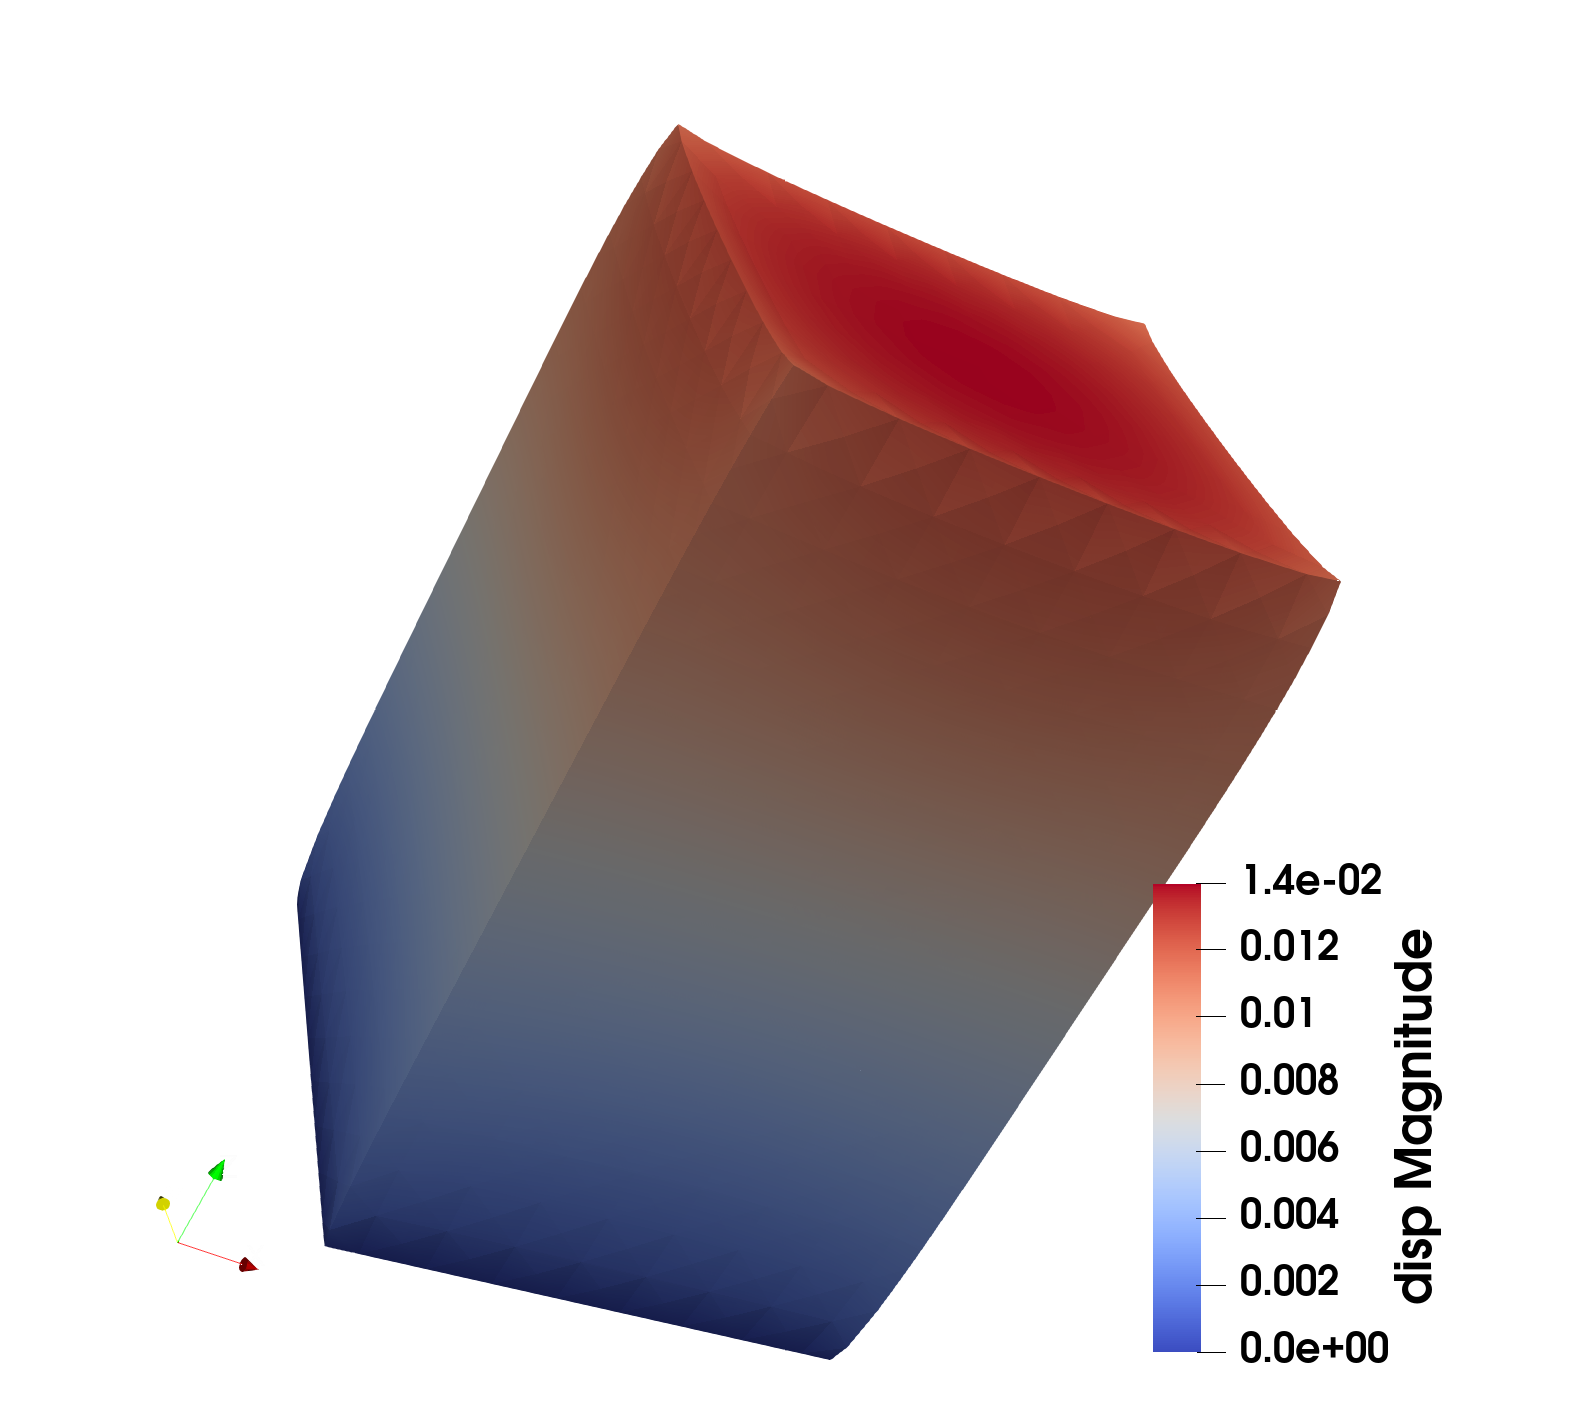
\includegraphics[width=0.46\linewidth]{./pic/mcc/conventional compression 100kpa-u.png}
			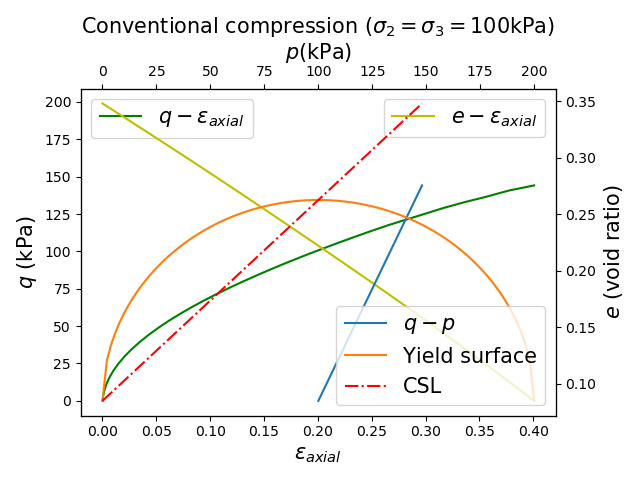
\includegraphics[width=0.52\linewidth]{./pic/mcc/conventional compression 100kpa.png}
			\caption{Conventional compression 3D}
			\label{fig: mcc conventional compression}
		\end{figure}
	\end{minipage}
	\begin{minipage}{0.48\linewidth}
		\begin{figure}
			\centering
			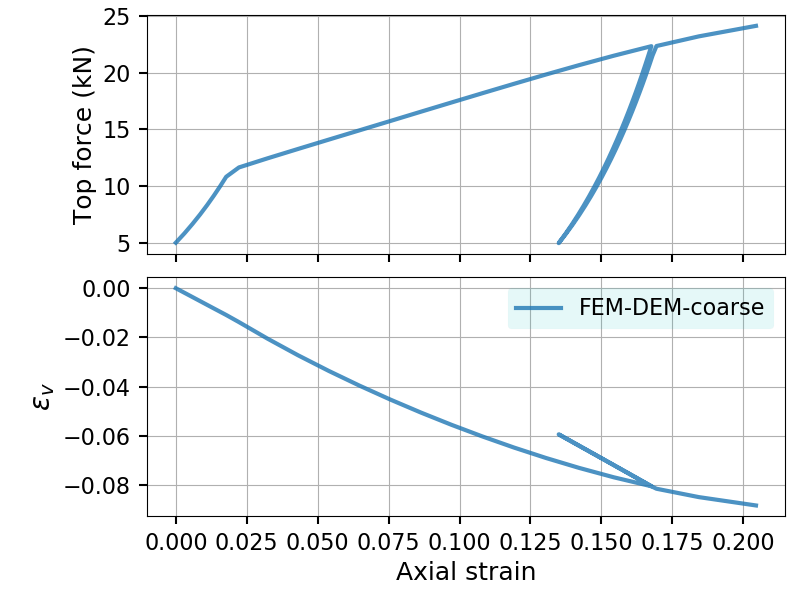
\includegraphics[width=0.48\linewidth]{./pic/mcc/biaxial_cylic_topforce.png}
			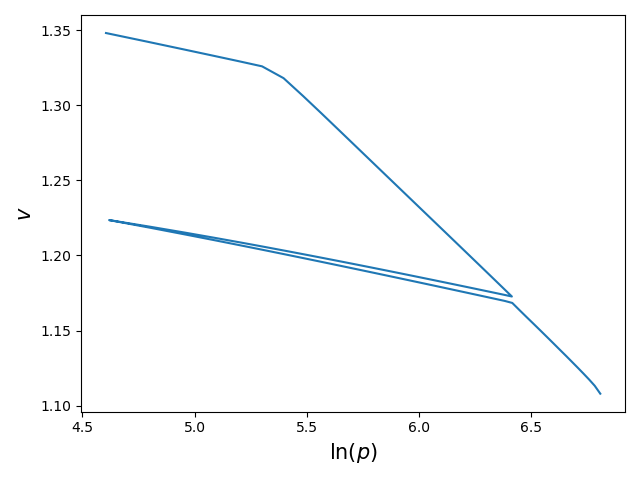
\includegraphics[width=0.48\linewidth]{./pic/mcc/cylic_consolidation.png}
			\caption{Cylic loading: (a) conventional compression; (b) isotropic compression}
			\label{fig: mcc cylic loading}
		\end{figure}
	\end{minipage}

\end{frame}

\begin{frame}{CSUH model}
	\fontsize{9}{9}\selectfont
	The model can describe the \textcolor{red}{dilation}, the \textcolor{red}{stress peak} and the \textcolor{red}{shearing band (strain localization)} of the dense sand (rockfill materials) in the conventioal compression simulations \textcolor{red}{($e_0=0.7$)}.
	
	\vspace{-2mm}
	\begin{minipage}[c]{0.46\linewidth}
		\fontsize{6}{6}\selectfont
		\begin{table}[]
			\caption{Parameters of the Toyoura sand}
			\begin{tabular}{ll}
				\hline
				Paramters & Value \\ \hline
				$M$       & 1.25  \\
				$\lambda$ & 0.135 \\
				$\kappa$  & 0.04  \\
				$v$       & 0.3   \\
				$N$       & 1.973 \\
				$e_{c0}$  & 0.934 \\
				$\chi$    & 0.4   \\
				$m$       & 1.8   \\ \hline
			\end{tabular}
		\end{table}
	\fontsize{6}{6}\selectfont
	
	\vspace{-6mm}
		\begin{figure}
			\centering
			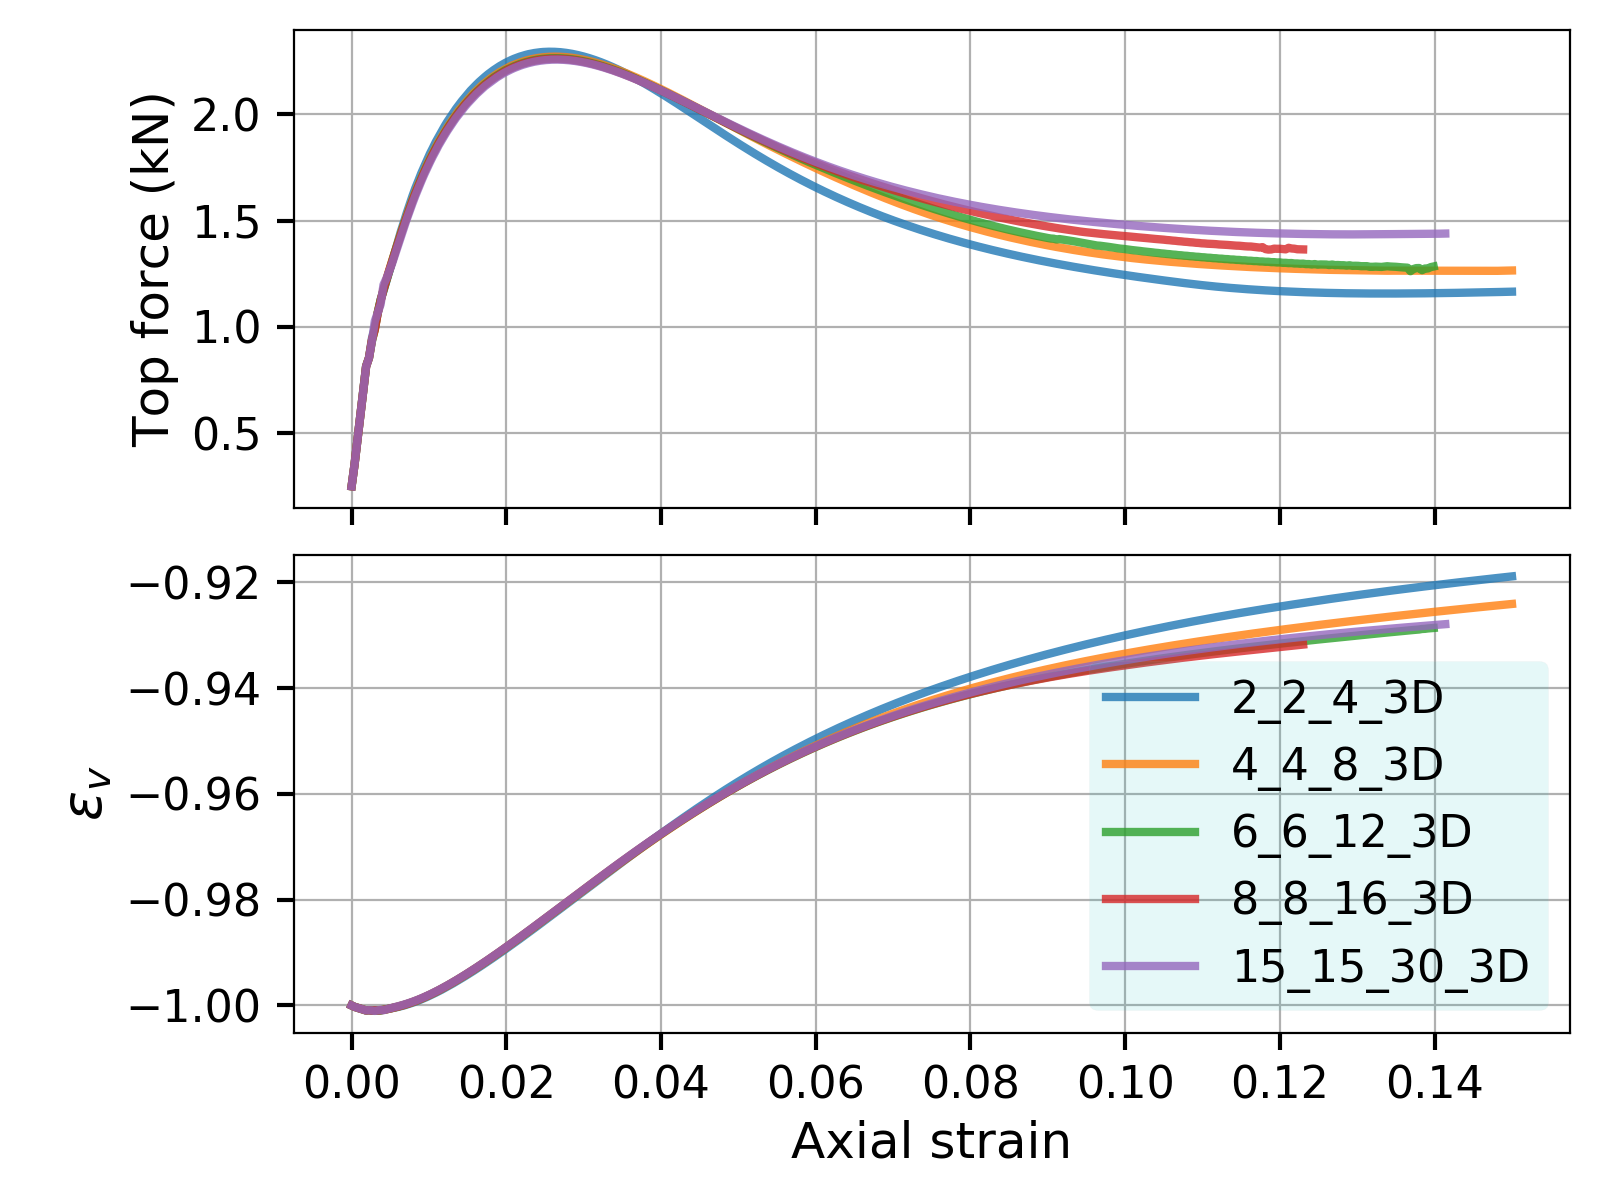
\includegraphics[width=0.65\linewidth]{./pic/csuh/conventional displacement compression_e0.png}
			\caption{Top force comparison}
			\label{fig: csuh conventional top force comparison}
		\end{figure}
	\end{minipage}
	\begin{minipage}[c]{0.52\linewidth}
		\begin{figure}
			\centering
			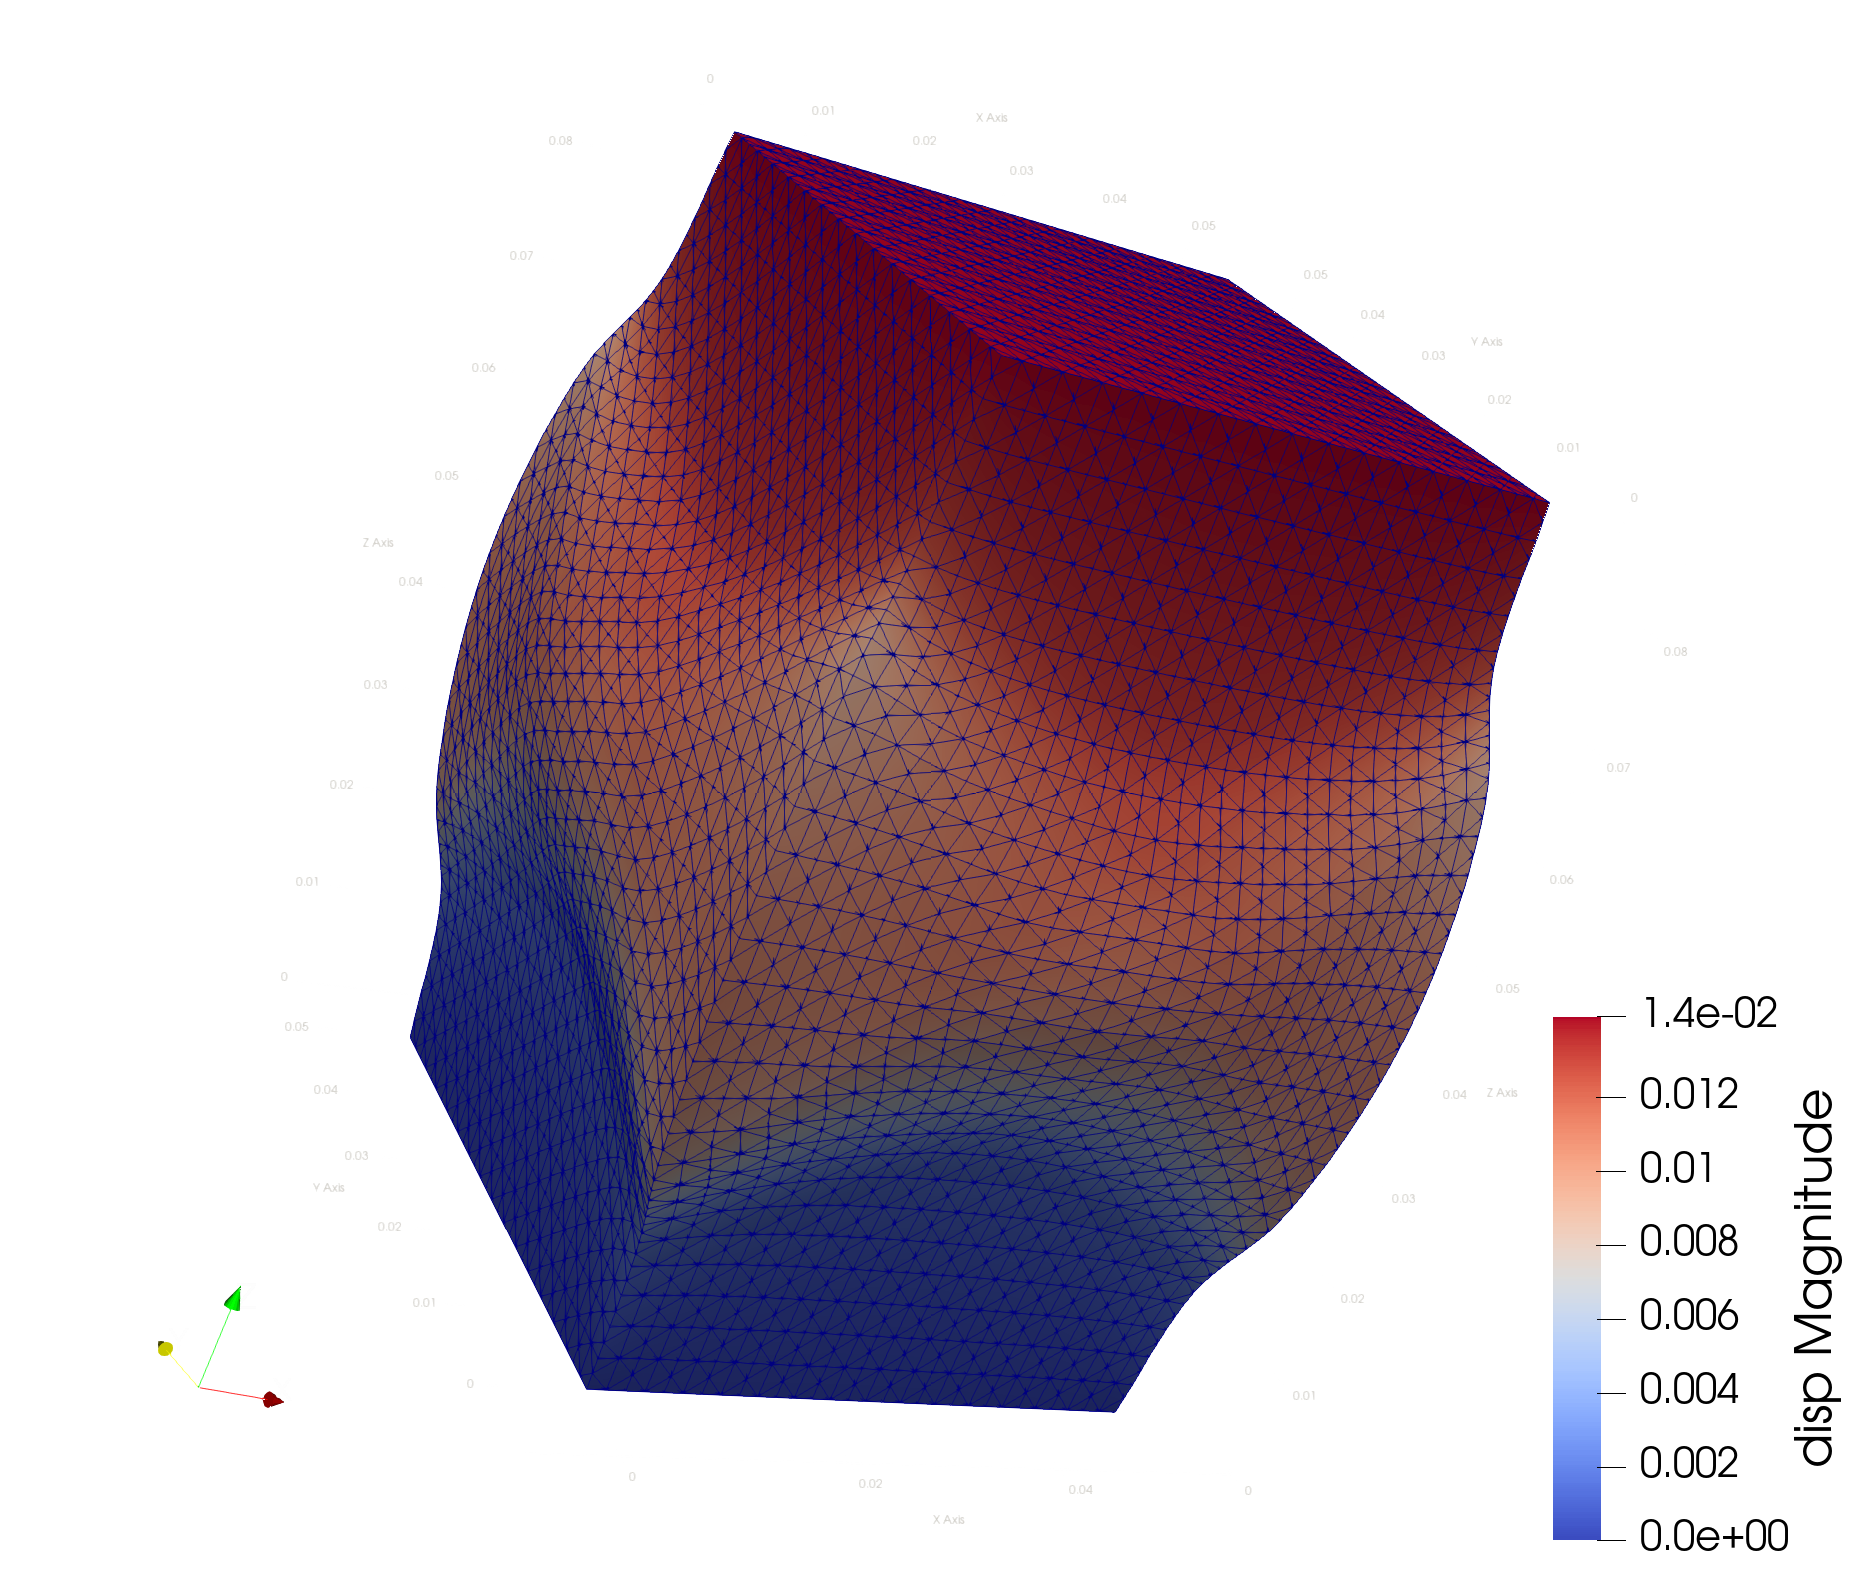
\includegraphics[width=0.47\linewidth]{./pic/csuh/e0.7_p0_1e5_dispMagtitude.png}
			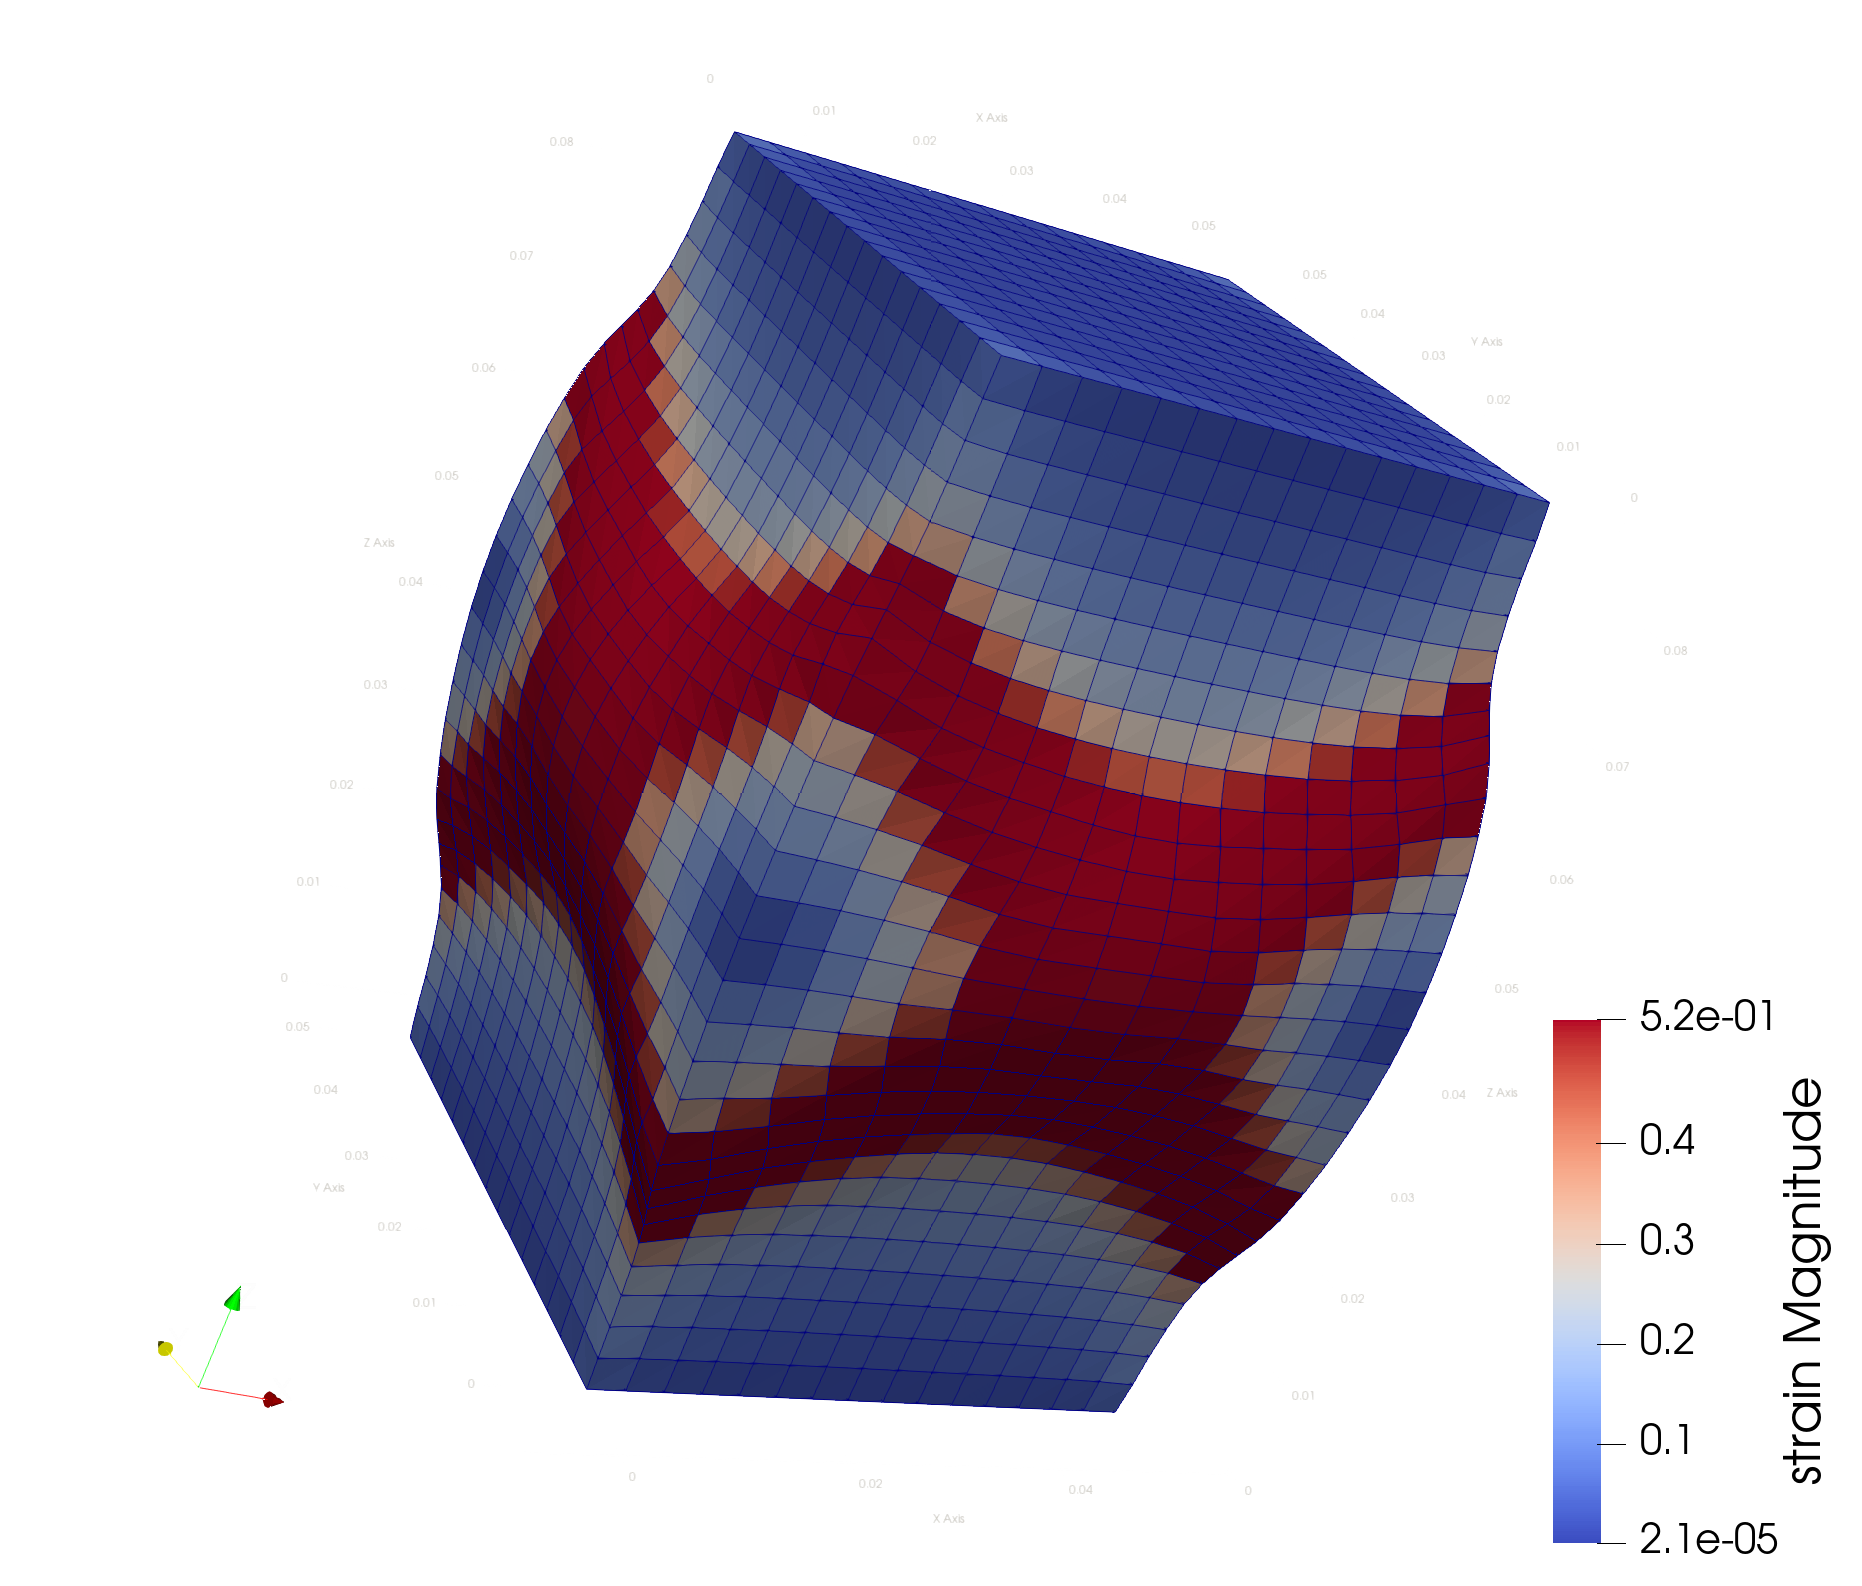
\includegraphics[width=0.47\linewidth]{./pic/csuh/e0.7_p0_1e5_epsMagtitude.png}
			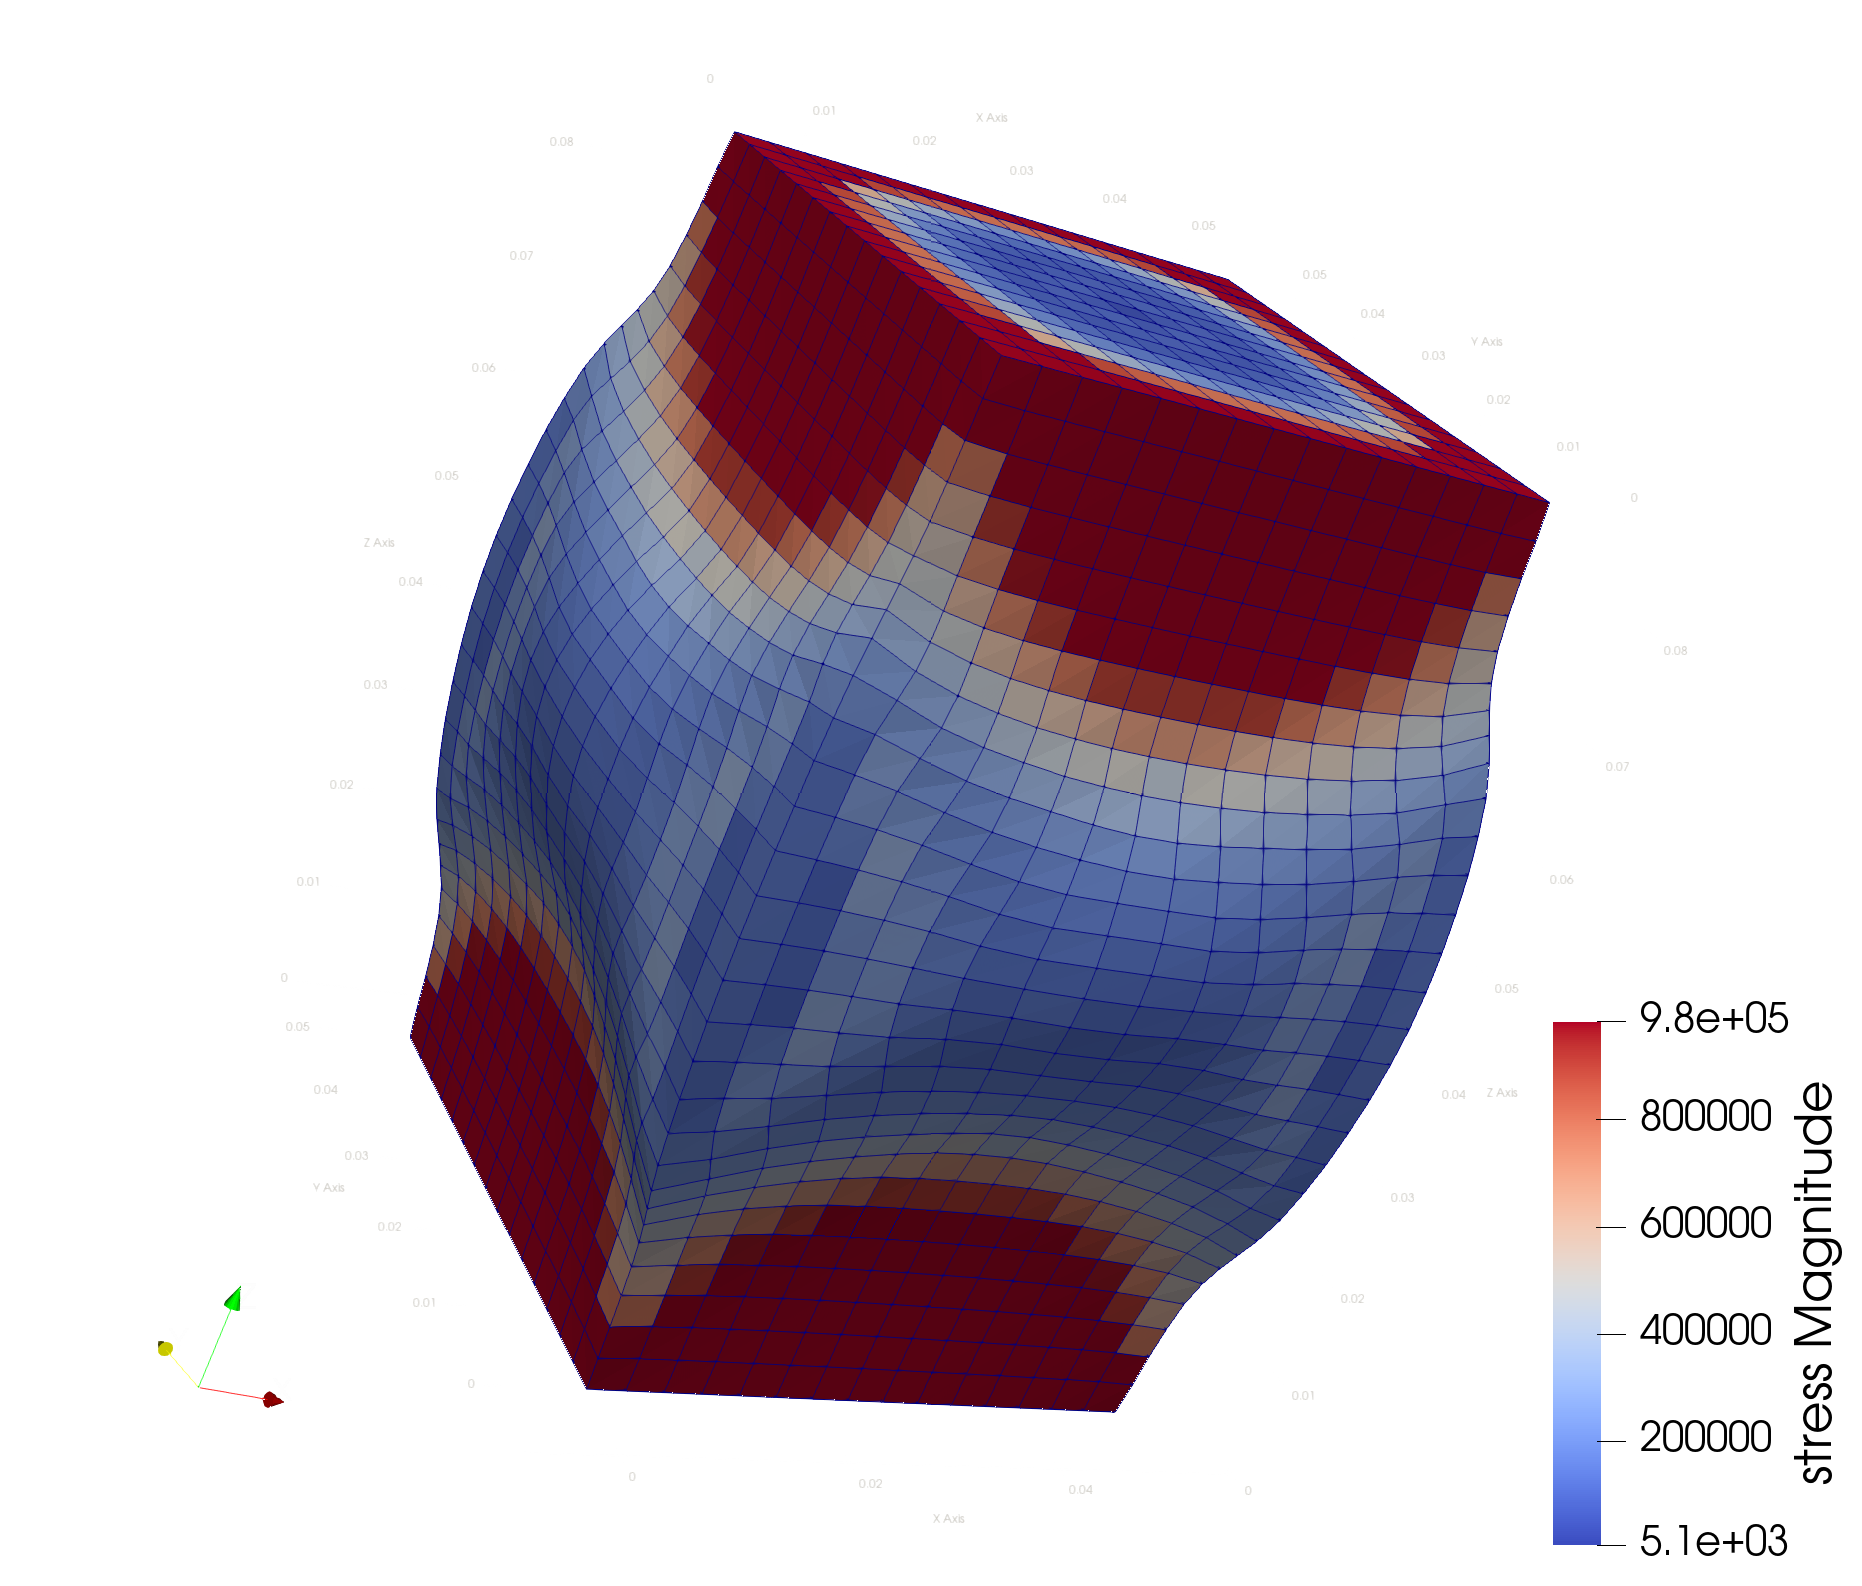
\includegraphics[width=0.47\linewidth]{./pic/csuh/e0.7_p0_1e5_sigMagtitude.png}
			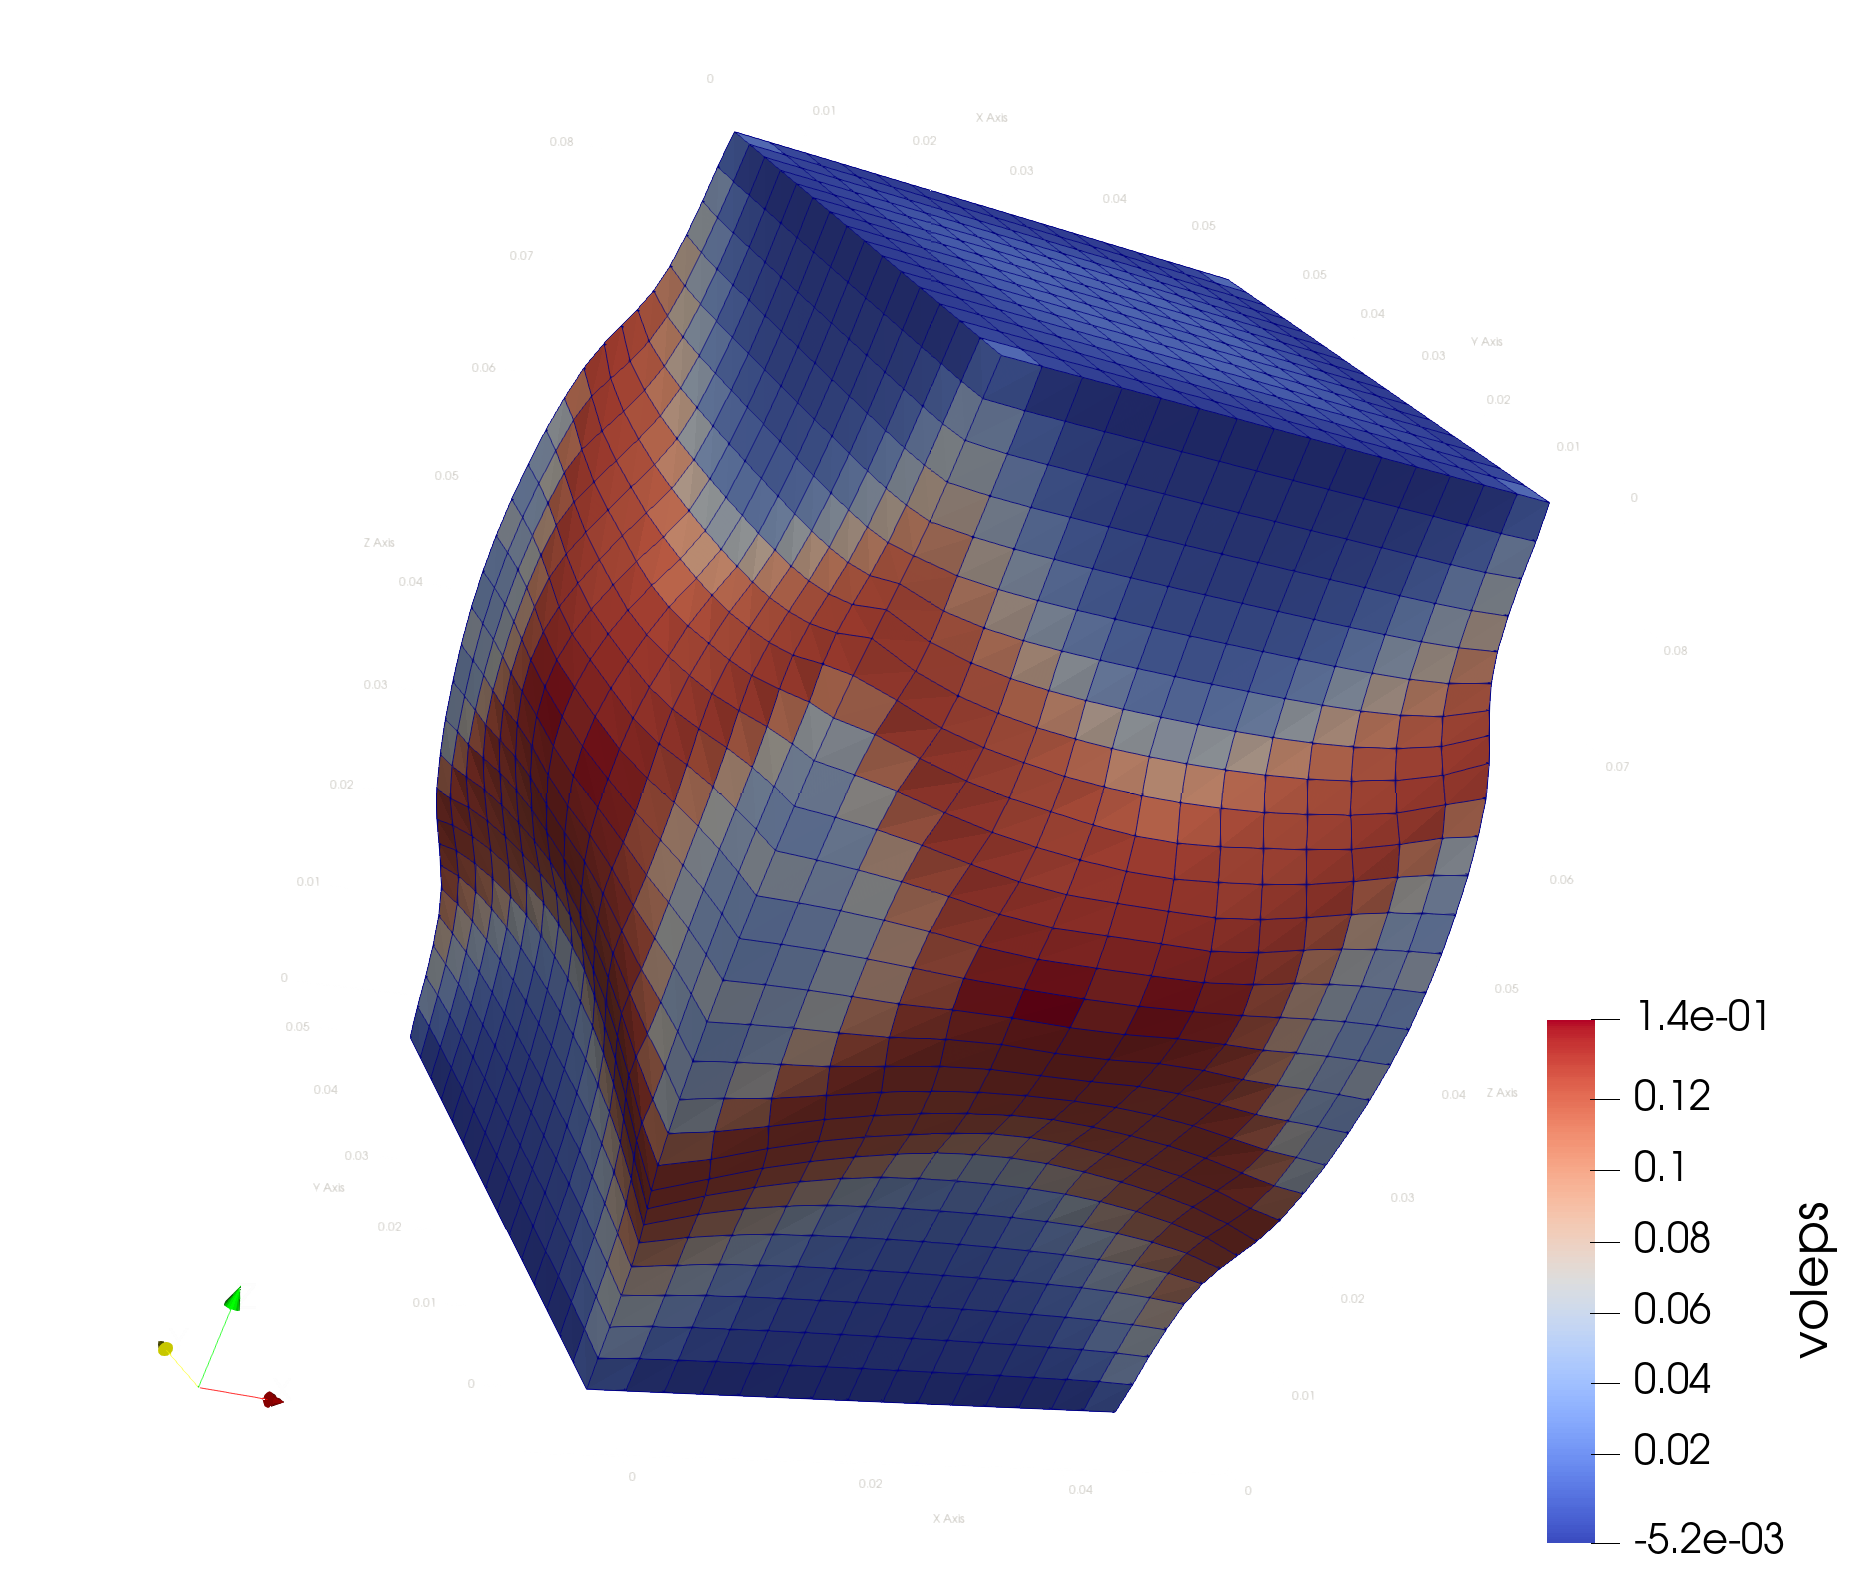
\includegraphics[width=0.47\linewidth]{./pic/csuh/e0.7_p0_1e5_volEps.png}
			\caption{Conventional compression 3D}
			\label{fig: csuh conventional compression}
		\end{figure}
	\end{minipage}

\end{frame}

%
%\section{why beamer}
%\begin{frame}{Why Beamer}
%    \begin{itemize}
%        \item \LaTeX 广泛用于学术界,期刊会议论文模板
%    \end{itemize}
%    \begin{table}[h]
%        \centering
%        \begin{tabular}{c|c}
%            Microsoft\textsuperscript{\textregistered}  Word & \LaTeX \\
%            \hline
%            文字处理工具 & 专业排版软件 \\
%            容易上手,简单直观 & 容易上手 \\
%            所见即所得 & 所见即所想,所想即所得 \\
%            高级功能不易掌握 & 进阶难,但一般用不到 \\
%            处理长文档需要丰富经验 & 和短文档处理基本无异 \\
%            花费大量时间调格式 & 无需担心格式,专心作者内容 \\
%            公式排版差强人意 & 尤其擅长公式排版 \\
%            二进制格式,兼容性差 & 文本文件,易读、稳定 \\
%            付费商业许可 & 自由免费使用 \\
%        \end{tabular}
%    \end{table}
%\end{frame}
%
%\begin{frame}{排版举例}
%    \begin{exampleblock}{无编号公式} % 加 * 
%        \begin{equation*}
%            J(\theta) = \mathbb{E}_{\pi_\theta}[G_t] = \sum_{s\in\mathcal{S}} d^\pi (s)V^\pi(s)=\sum_{s\in\mathcal{S}} d^\pi(s)\sum_{a\in\mathcal{A}}\pi_\theta(a|s)Q^\pi(s,a)
%        \end{equation*}
%    \end{exampleblock}
%    \begin{exampleblock}{多行多列公式\footnote{如果公式中有文字出现,请用 $\backslash$mathrm\{\} 或者 $\backslash$text\{\} 包含,不然就会变成 $clip$,在公式里看起来比 $\mathrm{clip}$ 丑非常多。}}
%        % 使用 & 分隔
%        \begin{align}
%            Q_\mathrm{target}&=r+\gamma Q^\pi(s^\prime, \pi_\theta(s^\prime)+\epsilon)\\
%            \epsilon&\sim\mathrm{clip}(\mathcal{N}(0, \sigma), -c, c)\nonumber
%        \end{align}
%    \end{exampleblock}
%\end{frame}
%
%\begin{frame}
%    \begin{exampleblock}{编号多行公式}
%        % Taken from Mathmode.tex
%        \begin{multline}
%            A=\lim_{n\rightarrow\infty}\Delta x\left(a^{2}+\left(a^{2}+2a\Delta x+\left(\Delta x\right)^{2}\right)\right.\label{eq:reset}\\
%            +\left(a^{2}+2\cdot2a\Delta x+2^{2}\left(\Delta x\right)^{2}\right)\\
%            +\left(a^{2}+2\cdot3a\Delta x+3^{2}\left(\Delta x\right)^{2}\right)\\
%            +\ldots\\
%            \left.+\left(a^{2}+2\cdot(n-1)a\Delta x+(n-1)^{2}\left(\Delta x\right)^{2}\right)\right)\\
%            =\frac{1}{3}\left(b^{3}-a^{3}\right)
%        \end{multline}
%    \end{exampleblock}
%\end{frame}
%
%\begin{frame}{图形与分栏}
%    % From thuthesis user guide.
%    \begin{minipage}[c]{0.3\linewidth}
%        \psset{unit=0.8cm}
%        \begin{pspicture}(-1.75,-3)(3.25,4)
%            \psline[linewidth=0.25pt](0,0)(0,4)
%            \rput[tl]{0}(0.2,2){$\vec e_z$}
%            \rput[tr]{0}(-0.9,1.4){$\vec e$}
%            \rput[tl]{0}(2.8,-1.1){$\vec C_{ptm{ext}}$}
%            \rput[br]{0}(-0.3,2.1){$\theta$}
%            \rput{25}(0,0){%
%            \psframe[fillstyle=solid,fillcolor=lightgray,linewidth=.8pt](-0.1,-3.2)(0.1,0)}
%            \rput{25}(0,0){%
%            \psellipse[fillstyle=solid,fillcolor=yellow,linewidth=3pt](0,0)(1.5,0.5)}
%            \rput{25}(0,0){%
%            \psframe[fillstyle=solid,fillcolor=lightgray,linewidth=.8pt](-0.1,0)(0.1,3.2)}
%            \rput{25}(0,0){\psline[linecolor=red,linewidth=1.5pt]{->}(0,0)(0.,2)}
%%           \psRotation{0}(0,3.5){$\dot\phi$}
%%           \psRotation{25}(-1.2,2.6){$\dot\psi$}
%            \psline[linecolor=red,linewidth=1.25pt]{->}(0,0)(0,2)
%            \psline[linecolor=red,linewidth=1.25pt]{->}(0,0)(3,-1)
%            \psline[linecolor=red,linewidth=1.25pt]{->}(0,0)(2.85,-0.95)
%            \psarc{->}{2.1}{90}{112.5}
%            \rput[bl](.1,.01){C}
%        \end{pspicture}
%    \end{minipage}\hspace{1cm}
%    \begin{minipage}{0.5\linewidth}
%        \medskip
%        %\hspace{2cm}
%        \begin{figure}[h]
%            \centering
%            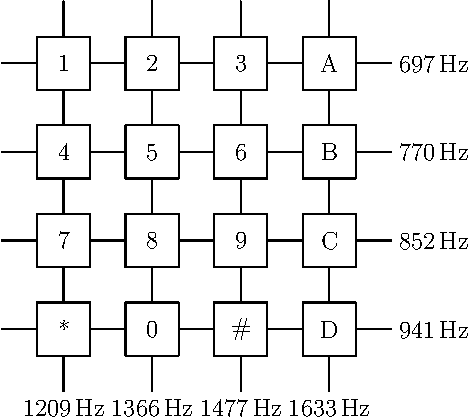
\includegraphics[height=.4\textheight]{pic/dtmf.pdf}
%        \end{figure}
%    \end{minipage}
%\end{frame}
%
%\begin{frame}[fragile]{\LaTeX{} 常用命令}
%    \begin{exampleblock}{命令}
%        \centering
%        \footnotesize
%        \begin{tabular}{llll}
%            \cmd{chapter} & \cmd{section} & \cmd{subsection} & \cmd{paragraph} \\
%            章 & 节 & 小节 & 带题头段落 \\\hline
%            \cmd{centering} & \cmd{emph} & \cmd{verb} & \cmd{url} \\
%            居中对齐 & 强调 & 原样输出 & 超链接 \\\hline
%            \cmd{footnote} & \cmd{item} & \cmd{caption} & \cmd{includegraphics} \\
%            脚注 & 列表条目 & 标题 & 插入图片 \\\hline
%            \cmd{label} & \cmd{cite} & \cmd{ref} \\
%            标号 & 引用参考文献 & 引用图表公式等\\\hline
%        \end{tabular}
%    \end{exampleblock}
%    \begin{exampleblock}{环境}
%        \centering
%        \footnotesize
%        \begin{tabular}{lll}
%            \env{table} & \env{figure} & \env{equation}\\
%            表格 & 图片 & 公式 \\\hline
%            \env{itemize} & \env{enumerate} & \env{description}\\
%            无编号列表 & 编号列表 & 描述 \\\hline
%        \end{tabular}
%    \end{exampleblock}
%\end{frame}
%
%\begin{frame}[fragile]{\LaTeX{} 环境命令举例}
%    \begin{minipage}{0.5\linewidth}
%\begin{lstlisting}[language=TeX]
%\begin{itemize}
%  \item A \item B
%  \item C
%  \begin{itemize}
%    \item C-1
%  \end{itemize}
%\end{itemize}
%\end{lstlisting}
%    \end{minipage}\hspace{1cm}
%    \begin{minipage}{0.3\linewidth}
%        \begin{itemize}
%            \item A
%            \item B
%            \item C
%            \begin{itemize}
%                \item C-1
%            \end{itemize}
%        \end{itemize}
%    \end{minipage}
%    \medskip
%    \pause
%    \begin{minipage}{0.5\linewidth}
%\begin{lstlisting}[language=TeX]
%\begin{enumerate}
%  \item 巨佬 \item 大佬
%  \item 萌新
%  \begin{itemize}
%    \item[n+e] 瑟瑟发抖
%  \end{itemize}
%\end{enumerate}
%\end{lstlisting}
%    \end{minipage}\hspace{1cm}
%    \begin{minipage}{0.3\linewidth}
%        \begin{enumerate}
%            \item 巨佬
%            \item 大佬
%            \item 萌新
%            \begin{itemize}
%                \item[n+e] 瑟瑟发抖
%            \end{itemize}
%        \end{enumerate}
%    \end{minipage}
%\end{frame}
%
%\begin{frame}[fragile]{\LaTeX{} 数学公式}
%    \begin{columns}
%        \begin{column}{.55\textwidth}
%\begin{lstlisting}[language=TeX]
%$V = \frac{4}{3}\pi r^3$
%
%\[
%  V = \frac{4}{3}\pi r^3
%\]
%
%\begin{equation}
%  \label{eq:vsphere}
%  V = \frac{4}{3}\pi r^3
%\end{equation}
%\end{lstlisting}
%        \end{column}
%        \begin{column}{.4\textwidth}
%            $V = \frac{4}{3}\pi r^3$
%            \[
%                V = \frac{4}{3}\pi r^3
%            \]
%            \begin{equation}
%                \label{eq:vsphere}
%                V = \frac{4}{3}\pi r^3
%            \end{equation}
%        \end{column}
%    \end{columns}
%    \begin{itemize}
%        \item 更多内容请看 \href{https://zh.wikipedia.org/wiki/Help:数学公式}{\color{purple}{这里}}
%    \end{itemize}
%\end{frame}
%
%\begin{frame}[fragile]
%    \begin{columns}
%        \column{.6\textwidth}
%\begin{lstlisting}[language=TeX]
%    \begin{table}[htbp]
%      \caption{编号与含义}
%      \label{tab:number}
%      \centering
%      \begin{tabular}{cl}
%        \toprule
%        编号 & 含义 \\
%        \midrule
%        1 & 4.0 \\
%        2 & 3.7 \\
%        \bottomrule
%      \end{tabular}
%    \end{table}
%    公式~(\ref{eq:vsphere}) 的
%    编号与含义请参见
%    表~\ref{tab:number}。
%\end{lstlisting}
%        \column{.4\textwidth}
%        \begin{table}[htpb]
%            \centering
%            \caption{编号与含义}
%            \label{tab:number}
%            \begin{tabular}{cl}\toprule
%                编号 & 含义 \\\midrule
%                1 & 4.0\\
%                2 & 3.7\\\bottomrule
%            \end{tabular}
%        \end{table}
%        \normalsize 公式~(\ref{eq:vsphere})的编号与含义请参见表~\ref{tab:number}。
%    \end{columns}
%\end{frame}
%
%\begin{frame}{作图}
%    \begin{itemize}
%        \item 矢量图 eps, ps, pdf
%        \begin{itemize}
%            \item METAPOST, pstricks, pgf $\ldots$
%            \item Xfig, Dia, Visio, Inkscape $\ldots$
%            \item Matlab / Excel 等保存为 pdf
%        \end{itemize}
%        \item 标量图 png, jpg, tiff $\ldots$
%        \begin{itemize}
%            \item 提高清晰度,避免发虚
%            \item 应尽量避免使用
%        \end{itemize}
%    \end{itemize}
%    \begin{figure}[htpb]
%        \centering
%        
\includegraphics[width=0.2\linewidth]{pic/whulogo.png}
%        \caption{这个校徽就是矢量图}
%    \end{figure}
%\end{frame}
%
%\section{templates}
%\begin{frame}
%    \begin{itemize}
%        \item 一月:完成文献调研
%        \item 二月:复现并评测各种Beamer主题美观程度
%        \item 三、四月:美化THU Beamer主题
%        \item 五月:论文撰写
%    \end{itemize}
%\end{frame}
%
%\begin{frame}
%    \begin{itemize}
%        \item 一月:完成文献调研
%        \item 二月:复现并评测各种Beamer主题美观程度
%        \item 三、四月:美化THU Beamer主题
%        \item 五月:论文撰写
%    \end{itemize}
%\end{frame}
%
%\section{Reference}
%

\begin{frame}[allowframebreaks]{Reference}
    \bibliography{ref}
    \tiny\bibliographystyle{alpha}
    % 如果参考文献太多的话,可以像下面这样调整字体:
    % \tiny\bibliographystyle{alpha}
\end{frame}

\begin{frame}
    \begin{center}
        {\Huge Thanks!}
    \end{center}
\end{frame}

\end{document}
